\documentclass[12pt,a4paper,UTF8,fontset=fandol]{ctexart}
\usepackage[margin=1in]{geometry}
\usepackage{amssymb,amsthm,mathtools}
\usepackage{algorithm,algpseudocode}
\usepackage{graphicx,subcaption,float}
\usepackage{booktabs,multirow,makecell}
\usepackage[numbers]{natbib}
\usepackage{hyperref}
\usepackage{xcolor}
\usepackage{enumitem}

\DeclareMathOperator*{\argmin}{arg\,min}
\DeclareMathOperator*{\argmax}{arg\,max}

\newtheorem{definition}{定义}[section]
\newtheorem{theorem}{定理}[section]
\newtheorem{lemma}{引理}[section]
\newtheorem{proposition}{命题}[section]
\newtheorem{corollary}{推论}[section]
\newtheorem{remark}{注记}[section]

\title{\textbf{博弈驱动的去中心化语义共识机制研究：\\基于AEIC分层分解与Stackelberg激励的多智能体框架}}
\author{马天成 \\ 指导教师：XXX教授}
\date{}

\begin{document}
\maketitle

%=============================================================
% 摘 要
%=============================================================
\begin{abstract}
大语言模型（LLM）驱动的多智能体系统正在成为解决复杂推理任务的核心范式，但如何将多个自主推理体的异构输出整合为可靠的集体判断——即\textbf{语义共识问题}——仍是该领域的核心瓶颈。现有方法存在根本性缺陷：均等投票范式（如ChatEval）在多数智能体错误时完全失效；无引导辩论范式受从众效应（sycophantic conformity）和共识坍缩（consensus collapse）困扰；中心化评估范式（如AgentVerse）依赖单一评估者，构成系统性单点故障。这些方法的共同症结在于将推理输出视为不可分解的原子单元，既无法定位分歧的语义来源，也缺乏激励智能体维持独立判断的机制。

本文提出\textbf{AEIC-Stackelberg}去中心化语义共识框架，从语义表示和激励机制两个层面系统性地解决上述问题。在语义层面，框架引入\textbf{AEIC语义分解协议}，将推理链解耦为假设（Assumption）、证据（Evidence）、推理（Inference）和结论（Conclusion）四个正交语义层，支持逐层相似度计算、精确冲突归因以及跨层一致性验证。基于此结构化表示，框架设计了\textbf{四组件复合信任评估机制}，通过推理-结论方向性一致性（IC）、证据-结论语义支持度（EC）、证据质量评估（EQ）和跨智能体证据共识度（EV）四个维度综合评估每个智能体的可信度——这是AEIC分层独有的检测能力，端到端方法无法实现。在激励层面，框架构建\textbf{Stackelberg博弈模型}，设计Leader-Follower激励结构驱动去中心化参数收敛，以博弈均衡参数$\theta$归一化后作为唯一投票权重，实现"信任评估驱动博弈参数$\to$博弈参数决定决策权重"的端到端链路。框架进一步支持六种多智能体通信模式（Parallel、Sequential、Star、Debate、SelfCorrect、AgentVerse），并引入17个可学习共识参数的数据驱动优化机制。

在StrategyQA、GSM-Hard、MMLU-Hard等10个推理基准数据集上，通过六项系统性实验从通信模式对比、参数优化、异构鲁棒性、信任组件消融、跨数据集泛化和可扩展性六个维度全面验证了框架的有效性。实验采用DeepSeek（强模型）和智谱GLM-4-Flash（弱模型/免费）两种异构LLM后端，结合本地Sentence-Transformer嵌入编码器，在真实LLM系统上进行端到端验证。

\noindent\textbf{关键词：} 多智能体语义共识；AEIC语义分解；Stackelberg博弈；去中心化协作；跨层信任评估；对抗鲁棒性
\end{abstract}

\tableofcontents
\newpage

%=============================================================
\section{引言}\label{sec:intro}
%=============================================================

\subsection{研究背景与动机}

大语言模型（Large Language Model, LLM）在自然语言理解、推理和生成方面展现出前所未有的能力~\cite{brown2020language,openai2023gpt4}，催生了以LLM为核心推理引擎的多智能体系统（Multi-Agent System, MAS）研究范式~\cite{wooldridge1995intelligent,talebirad2023multi,tran2025multi}。在这一范式中，多个LLM智能体围绕同一问题独立推理，通过协作达成超越单一智能体的集体决策能力。近期研究表明，多智能体协作在文本理解、代码生成、数学推理和工具使用等任务上均能取得显著的性能提升~\cite{chen2023agentverse,hong2023metagpt,wu2023autogen}。

然而，多智能体协作的核心瓶颈在于\textbf{共识机制}：当$N$个智能体就同一问题产生$N$个可能相互矛盾的推理结果时，系统如何将这些异构输出整合为单一可靠的集体判断？这一问题在传统分布式系统中已有深入研究——例如Paxos和Raft协议通过多数派投票解决节点间的数值一致性问题~\cite{olfati2007consensus}——但LLM智能体的语义共识面临本质上不同的挑战。与传统共识处理二值或数值状态不同，语义共识需要在高维、连续且具有复杂内部结构的自然语言推理链之间建立一致性，这使得经典的投票和复制策略不再适用。

多智能体语义共识的重要性不仅体现在性能指标上。在法律推理、医疗决策、金融分析等高风险应用场景中，集体判断的可靠性直接关系到决策质量。一个鲁棒的共识机制需要满足三个核心属性：\textbf{正确性}（正确的少数意见不应被错误的多数淹没）、\textbf{鲁棒性}（系统应对从众效应和对抗性操纵具有免疫力）以及\textbf{可解释性}（共识过程应能定位分歧来源并提供决策依据）。遗憾的是，现有方法在这三个维度上均存在显著不足。

\subsection{核心挑战}

多智能体语义共识问题的难度来源于以下三个相互交织的现实约束：

\textbf{（1）语义模糊性。}自然语言推理链是高维连续对象，蕴含丰富但模糊的语义信息。两个语义等价的推理可能采用完全不同的措辞和论证路径（"表述不同但语义一致"），而两个表述相似的推理可能在关键逻辑节点上存在本质分歧（"表述相似但语义矛盾"）。端到端的语义相似度计算将这两类情况混为一谈，导致虚假的高一致性信号或遗漏真正的语义冲突。

\textbf{（2）去中心化约束。}在隐私保护、大规模部署和抗审查等场景下，不存在全局可信的中央仲裁者。每个智能体仅能观察到直接通信邻居的信息，共识必须通过局部交互的迭代扩散来实现。这排除了依赖中央评估者的架构~\cite{chen2023agentverse}，要求共识机制具备分布式收敛的理论保证。

\textbf{（3）对抗性与从众效应。}多智能体系统面临两类威胁。第一类是模型幻觉（hallucination）~\cite{ji2023hallucination}：LLM可能生成事实错误但高度自信的推理链，导致"自信的错误"在投票中占据优势。第二类是从众效应（sycophantic conformity）：Bertalani\v{c}与Fortuna~\cite{bertalanic2026cost}的实证研究表明，在无引导辩论中，73\%的智能体会放弃自己的正确判断而采纳多数意见，正确答案被集体丢弃的比例（oracle gap）高达32\%。这两类威胁共同构成了对共识机制的严峻考验。

\subsection{现有方法的根本局限}\label{sec:limitation}

现有多智能体共识方法可归纳为三类范式，各存在根本性的结构缺陷：

\textbf{均等投票范式}，以ChatEval~\cite{chan2023chateval}为代表。该范式赋予所有智能体相同的决策权重，通过多数票决定最终结论。其致命缺陷在于：当多数智能体错误时（无论是因为模型幻觉还是系统性偏差），正确的少数意见被无条件丢弃。在我们构造的对抗性场景（2:1错误多数）中，ChatEval的Hard任务准确率为0\%——系统在最需要发挥作用的场景下完全失效。

\textbf{无引导辩论范式}，以Du等~\cite{du2023improving}和Liang等~\cite{liang2023encouraging}的工作为代表。同质智能体通过多轮讨论交换意见后投票。Bertalani\v{c}与Fortuna~\cite{bertalanic2026cost}的系统性实证研究揭示了三种失败模式：（i）\textbf{从众一致性}——73\%的智能体采纳多数答案而非坚持正确判断；（ii）\textbf{上下文脆弱性}——正确推理被同伴的不同观点干扰，15\%的正确智能体在辩论中转向错误；（iii）\textbf{共识坍缩}——最终投票中正确答案被丢弃，oracle gap高达32\%。该研究的核心结论是：在模型同质性的条件下，多轮辩论不仅未能提升共识质量，反而系统性地降低了准确率。

\textbf{中心化评估范式}，以AgentVerse~\cite{chen2023agentverse}为代表。中央评估者根据多维质量评分（证据覆盖度、推理连贯性、结论置信度）选择最佳智能体的结论。该范式在GPT-4驱动下表现出色，但存在结构性缺陷：评估者本身也是LLM实例，容易被高置信度的错误智能体误导——在我们的对抗性实验中，AgentVerse的评估者一致选择了"错误但自信"的智能体，Hard任务准确率同样为0\%。更根本地，单点评估构成系统的阿喀琉斯之踵——评估者一旦被误导，整个系统随之失效。

\textbf{三类范式的共同症结}可归结为一点：将推理输出视为不可分解的原子单元。在这一前提下，系统既无法定位分歧的具体语义来源（是证据不同、推理路径不同还是结论不同？），也无法验证推理链的内部一致性（推理方向是否与结论方向匹配？）。这种"语义黑箱"处理方式使得所有后续的聚合操作——无论是投票、辩论还是评估——都缺乏精确的语义基础。

\subsection{本文方法与贡献}

针对上述问题，本文提出\textbf{AEIC-Stackelberg去中心化语义共识框架}，从语义表示和激励机制两个层面进行系统性创新。

\textbf{核心思路。}本文的关键洞察是：如果将推理链视为"语义黑箱"，则任何聚合策略都无法区分"有价值的分歧"和"有害的从众"。解决方案是打开黑箱——将推理链分解为具有明确语义角色的结构化层次，在层次间建立一致性约束，并通过博弈论激励使智能体有动机维持独立判断。具体而言：
\begin{itemize}[nosep]
    \item \textbf{AEIC分解}将推理链解耦为假设（A）、证据（E）、推理（I）和结论（C）四个层次，使冲突定位和跨层验证成为可能；
    \item \textbf{跨层信任评估}利用AEIC的结构化特征——特别是推理方向（I）与结论方向（C）的一致性检测——识别被操纵或从众的智能体；
    \item \textbf{Stackelberg博弈}通过激励设计驱动去中心化参数收敛，保证共识的形成是激励相容的。
\end{itemize}

\textbf{主要贡献。}本文的具体贡献如下：

\begin{enumerate}[nosep]
    \item \textbf{AEIC语义分解协议}（第\ref{sec:framework}节）：提出将推理链解耦为四个正交语义层的结构化表示协议，支持逐层相似度计算和精确冲突归因，实现"靶向纠偏"式的共识优化。

    \item \textbf{四组件跨层信任评估机制}（第\ref{sec:trust}节）：设计IC（推理-结论方向性一致性，三层短路机制）、EC（证据-结论语义支持度）、EQ（证据质量评估）和EV（跨智能体证据共识度）四个互补组件，通过Stackelberg博弈间接形成决策权重。消融实验（第\ref{sec:exp4}节）验证了各组件的贡献。

    \item \textbf{六种通信模式与统一编排}（第\ref{sec:modes}节）：设计Parallel、Sequential、Star、Debate四种AEIC原生通信模式，并集成SelfCorrect和AgentVerse两种文献基线模式，通过$\sigma$注入机制实现AEIC层间信息传递与统一共识评估。

    \item \textbf{Stackelberg博弈收敛与纯$\theta$投票}（第\ref{sec:stackelberg}节）：设计Leader-Follower激励结构，以信任四维度构建投标参数，博弈均衡后$\theta$归一化为唯一投票权重。证明共识能量以$\exp(-2\gamma t/(N-1))$速率指数衰减。

    \item \textbf{17参数可学习共识配置}（第\ref{sec:experiments}节）：设计零API开销的两阶段参数优化流程（AEIC缓存收集$\to$差分进化全局优化），实现共识机制的数据驱动调优。

    \item \textbf{系统性实验验证}（第\ref{sec:experiments}节）：在10个推理基准数据集上，通过六项实验从通信模式对比、参数优化、异构鲁棒性、信任消融、跨数据集泛化和拓扑可扩展性六个维度全面验证框架有效性，所有实验基于真实LLM端到端执行。
\end{enumerate}

\subsection{论文组织}

本文的其余部分组织如下：第\ref{sec:related}节综述多智能体协作、辩论机制、博弈论应用和语义表示等相关研究；第\ref{sec:formulation}节形式化定义多智能体语义共识问题并阐述设计目标；第\ref{sec:framework}节系统阐述AEIC-Stackelberg框架的各组件设计；第\ref{sec:theory}节给出框架的理论分析，包括收敛性证明和复杂度分析；第\ref{sec:experiments}节报告六项实验的详细结果与分析；第\ref{sec:discussion}节讨论方法论意义和局限性；第\ref{sec:conclusion}节总结全文并展望未来研究方向。

%=============================================================
\section{相关工作}\label{sec:related}
%=============================================================

本节从五个方向综述与本文密切相关的研究，分析各方向的核心贡献与局限性，并阐明本文方法的定位。

\subsection{多智能体协作框架}

基于LLM的多智能体协作框架是近年来的研究热点。AgentVerse~\cite{chen2023agentverse}提出包含专家招募、协作决策、行动执行和评估反馈的四阶段框架，在多种任务上验证了多智能体协作优于单智能体的效果。MetaGPT~\cite{hong2023metagpt}将标准化操作流程（SOP）引入多智能体协作，通过角色分工和结构化通信提升软件开发任务的效率。AutoGen~\cite{wu2023autogen}提供了可定制的多智能体对话框架，支持灵活的智能体配置和人类参与模式。CAMEL~\cite{li2023camel}通过角色扮演（role-playing）范式驱动两个智能体围绕任务进行合作推理。ChatDev~\cite{qian2023chatdev}将软件开发流程建模为多智能体协作的通信链。Park等~\cite{park2023generative}则展示了生成式智能体在交互模拟环境中的涌现社会行为，揭示了多智能体协作的行为复杂性。

这些框架在协作架构设计上取得了重要进展，但在共识机制方面存在共同局限：要么依赖简单的多数投票（忽略智能体可信度差异），要么依赖中心化评估者（引入单点故障）。本文的AEIC-Stackelberg框架在共识机制这一核心环节上提供了结构化语义分解与博弈论激励的系统性创新，可作为上述框架的共识层替代方案。

\subsection{多智能体辩论与推理}

多智能体辩论是提升LLM推理可靠性的重要手段。Du等~\cite{du2023improving}的开创性工作表明，让多个LLM实例相互辩论、交换推理过程可以显著提升事实准确性和数学推理能力。Liang等~\cite{liang2023encouraging}进一步提出鼓励辩论中的发散性思维，以避免群体趋同。ChatEval~\cite{chan2023chateval}将多智能体辩论应用于文本质量评估，通过多轮讨论和投票提升评估的一致性和可靠性。

然而，Bertalani\v{c}与Fortuna~\cite{bertalanic2026cost}的系统性实证研究对上述乐观结论提出了重要修正。该研究在10个同质智能体、3轮辩论的设置下，揭示了三种根本性失败模式：\textbf{从众一致性}（73\%的智能体采纳多数答案）、\textbf{上下文脆弱性}（正确推理被同伴观点干扰）和\textbf{共识坍缩}（正确答案在最终投票中被丢弃）。其核心结论具有重要的理论意义：在模型同质且缺乏结构化引导的条件下，辩论无法保证共识质量的提升，甚至可能导致性能的系统性退化。

本文的设计直接回应了上述失败模式：AEIC分层分解对抗"缺乏结构化的从众"（智能体被迫在语义层面而非整体文本层面讨论分歧），Stackelberg激励对抗"缺乏维持独立意见的动机"（给予坚持独立判断的智能体更高的激励回报）。

\subsection{LLM推理增强}

LLM推理能力的提升是多智能体协作的基础。链式思维提示（Chain-of-Thought, CoT）~\cite{wei2022chain}通过在提示中加入中间推理步骤显著提升LLM在数学和逻辑推理任务上的表现。自一致性解码（Self-Consistency）~\cite{wang2023selfconsistency}通过采样多个推理路径并投票选择最一致的答案，提供了一种单模型内部的"共识"机制。思维树（Tree of Thoughts, ToT）~\cite{yao2023tree}将推理过程建模为树搜索，允许回溯和多路径探索。Reflexion~\cite{shinn2023reflexion}引入语言反馈机制使智能体从自身错误中学习。

这些方法关注单一模型的推理能力提升，本文则聚焦于多个异构模型之间的推理结果整合。两者具有互补性：更强的单体推理能力可以提升AEIC各层表示的质量，而AEIC-Stackelberg框架则确保多体推理结果的可靠聚合。值得注意的是，Self-Consistency可视为AEIC-Stackelberg在单模型多采样场景下的特例——但它缺乏跨层信任验证和博弈论激励，因此无法处理对抗性场景。

\subsection{博弈论与多智能体系统}

博弈论为多智能体行为建模提供了成熟的理论框架。Stackelberg博弈~\cite{stackelberg2011market}描述的Leader-Follower结构广泛应用于安全博弈、定价策略和资源分配等场景。演化博弈论~\cite{han2022emergent}通过选择压力和突变机制建模智能体群体的长期行为演化。分布式共识理论~\cite{olfati2007consensus}研究了网络化智能体如何通过局部信息交换达成全局一致。

本文的博弈论应用具有独特性：不同于传统Stackelberg博弈中Leader和Follower角色的固定分配，本文的Leader是"系统目标函数"（最大化全网对齐质量同时最小化共识能量），所有智能体均为Follower——它们根据激励参数决定对齐投入。这种设计使得博弈收敛等价于共识达成，从而将博弈论保证转化为共识保证。此外，本文将博弈论激励与语义信任评估耦合——信任分数决定了智能体在博弈中的初始参与阈值，高信任智能体获得更大的博弈权重，实现"结构化语义验证驱动激励分配"。

\subsection{语义相似度与LLM可靠性}

语义文本相似度（Semantic Textual Similarity, STS）是AEIC分层相似度计算的技术基础。Sentence-BERT~\cite{reimers2019sentence}通过对比学习微调BERT模型，生成适用于余弦相似度计算的句子嵌入，在STS-B等基准上取得了优异效果。本文采用多语言Sentence-Transformer（paraphrase-multilingual-MiniLM-L12-v2）作为嵌入编码器，在STS-B上验证Spearman $\rho = 0.854$。

LLM可靠性研究与本文的信任评估机制密切相关。Ji等~\cite{ji2023hallucination}对LLM幻觉现象进行了全面综述，指出事实不一致、逻辑矛盾和凭空编造是三种主要幻觉类型。Kadavath等~\cite{kadavath2022language}研究了LLM的自我知识边界感知能力，发现模型在校准（calibration）方面存在系统性偏差——尤其是过度自信倾向。这些发现为本文的置信度校准组件（Cal）提供了实证依据：当LLM表达高置信度但证据支撑不足时，很可能是幻觉或从众的产物。

%=============================================================
\section{问题形式化}\label{sec:formulation}
%=============================================================

本节形式化定义多智能体语义共识问题，建立符号约定，并阐述框架的设计目标。

\subsection{多智能体语义共识问题}

\begin{definition}[多智能体语义共识问题]\label{def:consensus}
给定任务描述$\mathcal{Q}$和$N$个自主推理智能体$\mathcal{A} = \{a_1, a_2, \ldots, a_N\}$，每个智能体独立生成推理结果$R_i = f_i(\mathcal{Q})$，其中$f_i$为智能体$i$的推理函数（由其底层LLM和推理策略决定）。\textbf{语义共识问题}是设计一个聚合机制$\mathcal{M}$，将$N$个推理结果映射为单一集体判断：
\begin{equation}
d^* = \mathcal{M}(R_1, R_2, \ldots, R_N; \mathcal{Q})
\end{equation}
使得$d^*$在给定的质量准则下最优。
\end{definition}

与传统分布式共识问题的关键区别在于：$R_i$不是简单的数值或二值状态，而是具有复杂内部结构的自然语言推理链，包含前提假设、事实证据、推理过程和最终结论等多个语义层次。

\subsection{符号约定}

表~\ref{tab:notation}汇总了本文使用的主要符号。

\begin{table}[H]
\centering
\caption{主要符号约定}\label{tab:notation}
\begin{tabular}{cl}
\toprule
符号 & 含义 \\
\midrule
$N$ & 智能体数量 \\
$R_i$ & 智能体$i$的推理结果 \\
$\langle A_i, E_i, I_i, C_i \rangle$ & $R_i$的AEIC四层分解 \\
$\phi(\cdot)$ & Sentence-Transformer编码函数 \\
$\mathbf{w} = [w_A, w_E, w_I, w_C]^\top$ & 各语义层的权重向量 \\
$\mathbf{v} = [v_A, v_E, v_I, v_C]^\top$ & softmax-logits参数向量 \\
$\text{IC}_i, \text{EC}_i, \text{EQ}_i, \text{EV}_i$ & 智能体$i$的四维信任评估分数 \\
$\theta_i$ & 智能体$i$的Stackelberg激励参数 \\
$\theta_{\text{norm},i}$ & 归一化后的投票权重 \\
$E$ & 共识能量（参数散度度量） \\
$w_{ij}$ & 网络拓扑权重 \\
$\gamma$ & 同伴压力系数 \\
$\eta$ & 学习率 \\
$\lambda$ & 能量惩罚系数 \\
\bottomrule
\end{tabular}
\end{table}

\subsection{设计目标}

本文提出的共识框架需要同时满足以下四个设计目标：

\textbf{D1 正确性（Correctness）。}当系统中存在正确推理时，集体判断$d^*$应倾向于正确结论，即使正确意见处于少数。形式化地，令$\mathcal{A}_{\text{correct}} \subseteq \mathcal{A}$为产出正确推理的智能体子集，设计目标是最小化oracle gap：
\begin{equation}
\text{OracleGap} = \Pr[\mathcal{A}_{\text{correct}} \neq \emptyset] - \Pr[d^* \text{ is correct}]
\end{equation}

\textbf{D2 鲁棒性（Robustness）。}系统应对从众效应和对抗性操纵具有容错能力。在至多$f < N/2$个智能体被操纵的条件下，集体判断仍应趋向正确。

\textbf{D3 去中心化（Decentralization）。}共识机制应能在无全局可信中央节点的条件下运行。每个智能体仅需与直接邻居通信，共识通过局部信息交换的迭代扩散形成。

\textbf{D4 效率（Efficiency）。}共识的通信复杂度和计算复杂度应随智能体数量$N$可控增长（至多多项式级），收敛轮数应在有限步内达成。

\subsection{对抗模型}

本文考虑以下对抗场景：

\begin{definition}[被动对抗模型]\label{def:adversary}
至多$f$个智能体（$f < N/2$）产生低质量或被操纵的推理结果。被操纵的智能体分为三个对抗等级：
\begin{itemize}[nosep]
    \item \textbf{Tier 1}（仅结论篡改）：结论$C_i$被翻转，但推理过程$I_i$保持原始方向——I$\to$C方向性检测可识别；
    \item \textbf{Tier 2}（结论+推理篡改）：$C_i$和$I_i$同时被修改——需要证据层分析（E$\to$C蕴含检测）；
    \item \textbf{Tier 3}（完全合理化）：$C_i$、$I_i$均被合理化改写，正确智能体的推理被模糊化——最困难的对抗等级。
\end{itemize}
\end{definition}

本文暂不考虑\textit{主动}对抗（恶意智能体刻意构造一致的假证据链），将其留作未来工作。

%=============================================================
\section{AEIC-Stackelberg 框架}\label{sec:framework}
%=============================================================

本节系统阐述AEIC-Stackelberg框架的各组件设计。框架的整体数据流如下：任务输入$\to$各智能体独立推理$\to$AEIC语义分解$\to$分层相似度计算与冲突归因$\to$自适应权重优化$\to$跨层信任评估$\to$Stackelberg博弈收敛$\to$信任加权投票$\to$集体判断输出。

\subsection{框架总览}

AEIC-Stackelberg框架由五个核心模块组成，各模块之间的关系如下：

\textbf{模块1：AEIC语义分解}（第\ref{sec:aeic}节）将推理链解耦为四层结构化表示，为后续所有分析提供语义基础。

\textbf{模块2：自适应权重学习}（第\ref{sec:adaptive}节）通过数据驱动优化确定各语义层在共识评估中的最优贡献权重。

\textbf{模块3：跨层信任评估}（第\ref{sec:trust}节）利用AEIC的层间结构验证每个智能体的内部一致性和外部可信度，生成复合信任分数。

\textbf{模块4：Stackelberg博弈}（第\ref{sec:stackelberg}节）以信任分数为输入，通过激励设计驱动智能体参数的去中心化收敛。

\textbf{模块5：去中心化网络}（第\ref{sec:network}节）提供P2P通信基础设施，支持分布式协议执行。

五个模块的设计体现了"语义结构$\to$信任评估$\to$博弈收敛$\to$集体决策"的渐进逻辑：AEIC分解提供语义结构，信任评估利用该结构甄别智能体，博弈收敛利用信任评估驱动参数对齐，最终通过耦合信任与博弈参数做出集体决策。

\subsection{AEIC 语义分解协议}\label{sec:aeic}

\begin{definition}[AEIC语义通信协议]
将智能体$i$的推理链$R_i$解耦为四个语义维度的结构化元组：
\begin{equation}
R_i = \langle A_i,\; E_i,\; I_i,\; C_i \rangle
\end{equation}
其中各层的语义角色定义如下：
\begin{itemize}[nosep]
    \item $A_i$（Assumption）：推理的前提假设与问题框架，定义了推理所处的假设空间；
    \item $E_i$（Evidence）：支撑推理的具体证据集合，$E_i = \{e_i^1, e_i^2, \ldots, e_i^{m_i}\}$；
    \item $I_i$（Inference）：从证据到结论的推理过程描述，包含逻辑推导和论证链；
    \item $C_i$（Conclusion）：最终判断或决策，是推理链的输出端。
\end{itemize}
\end{definition}

AEIC分解的设计遵循认知科学中的论证结构理论~\cite{fudenberg1991game}：一个完整的论证由假设前提、经验证据、推理过程和结论主张四个要素构成。这四个要素在认知功能上是正交的——假设定义了推理的边界条件，证据提供事实基础，推理建立从证据到结论的逻辑桥梁，结论是推理的产出。正交性意味着两个智能体可以在某些层面一致（如使用相同的证据）而在其他层面分歧（如推理路径不同），这为精确冲突定位提供了基础。

\subsubsection{分层相似度}

给定两个智能体$i, j$的推理记录，各层相似度定义为：
\begin{equation}
\text{sim}_X(R_i, R_j) = \text{CosSim}\bigl(\phi(X_i),\; \phi(X_j)\bigr), \quad X \in \{A, E, I, C\}
\end{equation}
其中$\phi(\cdot)$为Sentence-Transformer编码函数。对证据层，考虑到证据集合的集合性质，附加引用重叠度：
\begin{equation}
\text{sim}_E(R_i, R_j) = 0.6 \cdot \text{CosSim}(\phi(E_i), \phi(E_j)) + 0.4 \cdot \frac{|E_i \cap E_j|}{|E_i \cup E_j|}
\end{equation}

加权总相似度为：
\begin{equation}\label{eq:sim_aeic}
\text{SIM}_{\text{AEIC}}(R_i, R_j) = \sum_{X \in \{A,E,I,C\}} w_X \cdot \text{sim}_X(R_i, R_j)
\end{equation}
其中权重$\mathbf{w} = [w_A, w_E, w_I, w_C]^\top$满足$\sum_X w_X = 1$，$w_X > 0$。

\subsubsection{冲突归因}

AEIC分层的核心价值在于\textbf{精确定位分歧来源}：
\begin{equation}
\text{ConflictAttr}(i, j) = \argmin_{X \in \{A,E,I,C\}} \text{sim}_X(R_i, R_j)
\end{equation}

冲突归因使共识过程具备"靶向纠偏"能力——系统可针对分歧最严重的语义层组织讨论，而非全量打回所有层的内容。例如，若冲突主要源于证据层（两个智能体使用了不同的事实依据），则后续讨论应聚焦于证据的可靠性比较，而非重新审视假设或推理过程。

\subsubsection{AEIC相比端到端方法的优势}

端到端（E2E）方法将整个推理链拼接后计算单一相似度标量：
\begin{equation}
\text{SIM}_{\text{E2E}}(R_i, R_j) = \text{CosSim}\bigl(\phi(\text{concat}(R_i)),\; \phi(\text{concat}(R_j))\bigr)
\end{equation}

E2E方法存在三个结构性缺陷：（1）无法定位冲突源——一个标量无法回答"分歧在哪里"；（2）长文本中局部差异被稀释——当推理链较长时，某个层的关键分歧可能被其他层的高一致性掩盖；（3）无法实施差异化信任评估——所有层被等同对待，无法基于特定层（如IC方向性一致性）的结构信号区分智能体质量。第\ref{sec:experiments}节的实验定量验证了AEIC分层结构在信任评估和共识决策中的优势。

\subsection{自适应权重学习}\label{sec:adaptive}

\subsubsection{Softmax-Logits参数化}

权重向量$\mathbf{w}$的直接优化面临约束满足问题（非负性和归一化）。本文采用softmax-logits参数化规避此问题：定义可学习参数$\mathbf{v} = [v_A, v_E, v_I, v_C]^\top \in \mathbb{R}^4$，通过softmax映射为权重：
\begin{equation}\label{eq:softmax}
w_X = \frac{\exp(v_X)}{\sum_{Y \in \{A,E,I,C\}} \exp(v_Y)}
\end{equation}

该参数化自动满足$w_X > 0$和$\sum_X w_X = 1$，且在梯度优化中无需投影步。初始化$\mathbf{v} = \mathbf{0}$对应均匀权重$w_X = 0.25$。

\subsubsection{效用驱动的权重更新}

定义单轮效用函数：
\begin{equation}
U(t) = \overline{\text{sim}}(t) \cdot R - C
\end{equation}
其中$\overline{\text{sim}}(t) = \frac{1}{\binom{N}{2}} \sum_{i<j} \text{SIM}_{\text{AEIC}}(R_i, R_j)$为全网平均相似度，$R$为奖励系数，$C$为固定成本。

logits更新规则：
\begin{equation}\label{eq:weight_update}
v_X^{(t+1)} = v_X^{(t)} + \eta \cdot \frac{d_X^{(t)}}{\sum_Y d_Y^{(t)}} \cdot \max\!\left(\frac{U(t)}{R},\; 0.01\right)
\end{equation}
其中$d_X^{(t)} = \frac{1}{\binom{N}{2}} \sum_{i<j} \text{sim}_X^{(t)}(R_i, R_j)$为第$X$层的平均相似度（维度贡献度），$\eta$为学习率。

该更新规则的直觉是\textbf{自强化}：高一致性的层获得更大的权重提升（因为该层的一致性信号对共识贡献更大），而低一致性的层被抑制。系统通过迭代自动学习"哪些层对共识判断的贡献最大"。

\subsection{跨层信任评估机制}\label{sec:trust}

跨层信任评估是本框架的核心创新——它利用AEIC的结构化分层实现"对抗性场景下的少数正确识别"。核心思想是：一个可信的推理链，其四个语义层之间应满足特定的一致性约束；当这些约束被违反时，表明该智能体的推理可能被操纵或产生于从众效应。本框架设计了四个互补的信任组件：IC（推理-结论方向性一致性）、EC（证据-结论语义支持度）、EQ（证据质量）和EV（跨智能体证据共识度）。

\subsubsection{IC：推理-结论方向性一致性}

\begin{definition}[推理-结论一致性]\label{def:ic}
IC组件检测推理层$I_i$与结论层$C_i$之间的方向性语义对齐度。实现采用三层短路机制（优先级递减）：

\textbf{层1：共享概念对齐。}检测$I_i$和$C_i$是否共享相同的关键方向性概念。当两者包含相同的信号词（如"impossible"、"cannot"、"支持"等），且共享比例超过阈值$\tau_c = 0.3$时，判定为语义一致：
\begin{equation}
\text{ConceptAlign}(I_i, C_i) = \frac{|\mathcal{K}(I_i) \cap \mathcal{K}(C_i)|}{\min(|\mathcal{K}(I_i)|, |\mathcal{K}(C_i)|)}
\end{equation}
其中$\mathcal{K}(\cdot)$为从文本中提取的方向性信号词集合（包含中英文正/负方向信号词共70余个）。若$\text{ConceptAlign} > \tau_c$，则$d_{\text{IC}} = 0.7 + 0.2 \cdot \min(\text{ConceptAlign}, 1)$。

\textbf{层2：结论段方向匹配。}当层1未触发时，提取$I_i$中结论性语句段落——即最后一个过渡标志词（如"因此"、"therefore"、"综上"等）之后的文本——仅对该段落进行方向性检测：
\begin{equation}
d_{\text{IC}} = \begin{cases}
0.8 + 0.2 \cdot \text{conf} & \text{若结论段方向} = s(C_i) \\
0.2 - 0.1 \cdot \text{conf} & \text{若结论段方向} \neq s(C_i) \\
0.5 & \text{若无可检测方向信号}
\end{cases}
\end{equation}
其中$\text{conf} = |n_{\text{pos}} - n_{\text{neg}}| / (n_{\text{pos}} + n_{\text{neg}})$为方向检测置信度，$s(C_i) \in \{\text{yes}, \text{no}, \text{neutral}\}$为结论立场。

\textbf{层3：语义相似度兜底。}当前两层均无法提供方向性信号时，$d_{\text{IC}} = 0.5$（中性基线）。
\end{definition}

最终IC分数融合方向性得分与语义嵌入相似度：
\begin{equation}\label{eq:ic}
\text{IC}_i = 0.5 \cdot d_{\text{IC}} + 0.5 \cdot \text{CosSim}(\phi(I_i), \phi(C_i))
\end{equation}

\textbf{设计动机。}三层机制解决了传统方向检测的核心难题——\textit{双重否定场景}。例如，对问题"Is X impossible?"，诚实智能体的推理可能包含大量否定词（"cannot"、"no evidence"），但结论为"Yes: it is impossible"。传统全文方向检测会将推理判定为负向（否定词占多数），与正向结论矛盾，导致误判。三层机制通过共享概念对齐（层1，检测到I和C都提及"impossible/cannot"）或结论段聚焦（层2，仅看"因此，答案是肯定的"这一结论段）避免此类误判。

\subsubsection{EC：证据-结论语义支持度}

EC组件检测证据内容$E_i$是否在方向性和语义上支持结论$C_i$，融合方向匹配与语义相似度：
\begin{equation}\label{eq:ec}
\text{EC}_i = 0.5 \cdot d_{\text{EC}} + 0.5 \cdot \text{CosSim}(\phi(E_i), \phi(C_i))
\end{equation}
其中方向性得分$d_{\text{EC}}$通过检测证据文本整体方向与结论立场的匹配程度确定：
\begin{equation}
d_{\text{EC}} = \begin{cases}
0.85 & \text{若 } \text{dir}(E_i) = s(C_i) \\
0.15 & \text{若 } \text{dir}(E_i) \neq s(C_i) \\
0.5 & \text{若任一方向为中性}
\end{cases}
\end{equation}

\textbf{物理意义。}EC检测"证据与结论之间的语义断裂"——当证据讨论的事实指向X但结论声称Y时，EC分数降低。与IC的区别在于：IC关注推理过程的\textit{方向性逻辑一致性}（推理方向是否指向结论），而EC关注\textit{事实证据的语义支撑强度}（证据是否蕴含结论）。两者分别对应逻辑层面和事实层面的一致性验证。在对抗场景中，被篡改的智能体可能具有一致的I$\to$C方向（如Tier 2攻击中推理和结论同时被修改），但其原始证据仍可能指向真实答案——此时EC提供额外的检测能力。

\subsubsection{EQ：证据质量评估}

EQ组件衡量证据集合$E_i$的具体性和信息密度，不依赖跨智能体比较，仅评估单个智能体证据的内在质量。从四个维度综合评估：
\begin{equation}\label{eq:eq}
\text{EQ}_i = 0.2 \cdot \text{ItemCount}_i + 0.3 \cdot \text{Length}_i + 0.3 \cdot \text{Density}_i + 0.2 \cdot \text{Diversity}_i
\end{equation}
其中：
\begin{itemize}[nosep]
    \item $\text{ItemCount}_i = \min(|E_i| / 3,\; 1)$：证据条数（多条独立证据优于单条笼统陈述）；
    \item $\text{Length}_i = \min(\bar{\ell}_i / 60,\; 1)$：证据平均字符长度（具体事实通常更长）；
    \item $\text{Density}_i$：信息密度，统计证据中包含的数字、年份（$\backslash$d\{4\}）、百分比和专有名词的频率；
    \item $\text{Diversity}_i$：证据多样性，通过比较各条证据开头的独特性衡量不重复度。
\end{itemize}

\textbf{设计动机。}在异构多智能体场景中，强模型（如DeepSeek-V3）倾向于提供具体的事实、数据和引用，而弱模型（如GLM-4-Flash等免费模型）倾向于给出笼统的概括性陈述。EQ通过量化这种差异，为后续的Stackelberg博弈提供基于证据质量的区分信号——高EQ的智能体在投标构建中获得更高的对齐意愿度。

\subsubsection{EV：跨智能体证据共识度}

EV组件衡量智能体$i$的证据与通信邻居证据的语义一致性：
\begin{equation}\label{eq:ev}
\text{EV}_i = \frac{1}{|\mathcal{N}(i)|} \sum_{j \in \mathcal{N}(i)} \text{CosSim}(\phi(E_i), \phi(E_j))
\end{equation}
其中$\mathcal{N}(i)$为智能体$i$的通信邻居集合。在全连接拓扑下$\mathcal{N}(i) = \mathcal{A} \setminus \{i\}$；在稀疏拓扑（如Ring、Star）下仅包含直接邻居。

\textbf{物理意义。}当多个独立智能体基于相同的事实基础产出证据时，高EV表明该智能体使用了可靠的、被多方印证的事实证据。使用异常证据（如凭空捏造的事实或与所有其他智能体完全不同的信息源）的智能体将获得较低的EV分数。EV在Parallel模式下尤为重要：当所有智能体独立推理时，证据的交叉验证是判断事实可靠性的关键信号。在Sequential模式下，EV替换为证据新颖度（Evidence Novelty），衡量后续智能体提供的新信息量——此时新颖性而非重复性更具价值。

\subsubsection{从信任评估到博弈投标}

与传统的加权求和信任分数不同，本框架不直接将IC、EC、EQ、EV合并为标量信任分数用于投票。相反，四个维度通过可学习的参数映射构建Stackelberg博弈的投标参数（详见第\ref{sec:stackelberg}节）：
\begin{align}
\text{AlignWill}_i &= \max\!\left(\delta_{\text{aw}},\; \text{IC}_i^{\beta_1} \cdot \text{EQ}_i^{\beta_2} \cdot (\beta_3 + \beta_4 \cdot \text{EV}_i)\right) \label{eq:bid_aw} \\
\text{RevCost}_i &= \max\!\left(\delta_{\text{rc}},\; \beta_5 \cdot (1 - \text{Agree}_i)\right) \label{eq:bid_rc} \\
\text{MaxDepth}_i &= \text{clip}(\text{EC}_i,\; \beta_6,\; \beta_7) \label{eq:bid_mrd} \\
\text{HistAlign}_i &= \beta_8 \cdot \text{IC}_i + \beta_9 \cdot \text{EC}_i + \beta_{10} \cdot \text{EQ}_i + \beta_{11} \cdot \text{EV}_i \label{eq:bid_ha}
\end{align}
其中$\{\beta_k\}$和$\{\delta\}$为可学习参数（共12个投标构建参数 + 4个Stackelberg博弈参数 + 1个对齐下限 = 17个参数，详见第\ref{sec:exp2}节的参数优化实验），$\text{Agree}_i$为智能体$i$与邻居的立场一致率。这一参数化设计使得信任评估到最终决策的完整映射链路均可通过数据驱动优化，而非依赖手工设定的固定权重。

\subsection{Stackelberg 博弈收敛机制}\label{sec:stackelberg}

\subsubsection{共识能量}

定义全网共识能量为激励参数的二次散度：
\begin{equation}\label{eq:energy}
E = \frac{1}{2} \sum_{i<j} w_{ij}\,(\theta_i - \theta_j)^2
\end{equation}
其中$\theta_i \in (0,1)$为智能体$i$的激励参数（表征其对齐意愿度），$w_{ij}$为网络拓扑权重。$E \to 0$表示所有智能体的对齐投入趋于一致——即共识在参数空间中达成。

\subsubsection{Leader-Follower结构}

\textbf{Follower效用函数。}智能体$i$观察激励$\theta_i$后选择对齐投入$\alpha_i$：
\begin{equation}
U_i(\alpha_i;\, \theta_i) = \theta_i \cdot q_i(\alpha_i) \cdot R - c_i \cdot \alpha_i
\end{equation}
其中对齐质量函数$q_i(\alpha_i) = h_i \cdot \min(\alpha_i / \kappa_i,\; \kappa_i / \alpha_i)$为凹函数（先增后减），$h_i$为历史对齐率（由式\eqref{eq:bid_ha}的$\text{HistAlign}_i$确定），$\kappa_i$为能力上限（由式\eqref{eq:bid_mrd}确定），$c_i$为修改成本（由式\eqref{eq:bid_rc}确定）。

\begin{theorem}[Follower最优响应]\label{thm:follower}
智能体$i$的最优对齐投入为：
\begin{equation}
\alpha_i^*(\theta_i) = \kappa_i \cdot \min\!\left(\frac{\theta_i}{\tau_i},\; 1\right), \quad \tau_i = \frac{c_i \kappa_i}{h_i R}
\end{equation}
其中$\tau_i$为参与阈值——只有当激励超过阈值时智能体才全力对齐。
\end{theorem}

\textbf{Leader目标函数。}系统层面（Leader）的目标是最大化全网对齐质量，同时约束共识能量和预算：
\begin{equation}\label{eq:leader}
\max_{\boldsymbol\theta}\; \mathcal{J}(\boldsymbol\theta) = \sum_{i=1}^N q_i(\alpha_i^*(\theta_i)) - \lambda\,E - \mu \sum_{i=1}^N \theta_i
\end{equation}
其中$\lambda$为能量惩罚系数，$\mu$为预算约束系数。

\subsubsection{分布式更新规则}

激励参数通过梯度上升与同伴压力联合更新：
\begin{equation}\label{eq:theta_update}
\theta_i^{(t+1)} = \theta_i^{(t)} + \eta\,\frac{\partial \mathcal{J}}{\partial \theta_i} - \gamma \sum_{j \neq i} w_{ij}(\theta_i^{(t)} - \theta_j^{(t)})
\end{equation}
其中$\eta$为学习率，$\gamma$为同伴压力系数。更新规则中的两个力的物理含义是：梯度项驱动每个智能体向局部最优对齐方向移动，同伴压力项（本质上是图拉普拉斯扩散算子）驱动参数向全局均值收敛。两者的联合作用确保了"个体最优"与"全局一致"的平衡。

\subsubsection{纯$\theta$归一化投票}

在本框架中，Stackelberg博弈收敛后的均衡参数$\theta_i^*$被归一化至$[0,1]$后作为\textbf{唯一}投票权重：
\begin{equation}\label{eq:theta_norm}
\theta_{\text{norm},i} = \frac{\theta_i^* - \min_j \theta_j^*}{\max_j \theta_j^* - \min_j \theta_j^*}
\end{equation}

最终决策为：
\begin{equation}\label{eq:decision}
\text{Decision} = \arg\max_{s \in \mathcal{S}} \sum_{i:\, s(C_i)=s} \theta_{\text{norm},i}
\end{equation}
其中$\mathcal{S}$为所有立场的集合（$\{\text{yes}, \text{no}\}$）。

\textbf{设计理由。}与传统方法使用$\hat{T}_i \cdot \theta_i^*$的乘积权重不同，本框架采用纯$\theta_{\text{norm}}$投票。关键洞察在于：IC、EC、EQ、EV四个信任维度的信息已通过投标构建（式\eqref{eq:bid_aw}--\eqref{eq:bid_ha}）完整编码进Stackelberg博弈的输入参数中，博弈均衡过程已将这些信任信号与网络拓扑、激励约束融合为最优的$\theta^*$分配。再额外乘以$\hat{T}_i$将导致信任信号的\textit{双重计算}——一方面通过投标影响$\theta^*$，另一方面直接参与投票权重。纯$\theta_{\text{norm}}$设计确保了信任信号通过单一路径（投标$\to$博弈$\to\theta$）影响决策，语义清晰且避免冗余。

\subsection{去中心化网络协议}\label{sec:network}

\subsubsection{系统架构}

系统采用P2P拓扑，由轻量注册中心辅助初始发现：
\begin{itemize}[nosep]
    \item \textbf{注册中心}（Registry）：维护在线智能体表，提供节点发现服务，\textbf{不参与}共识计算；
    \item \textbf{智能体节点}（AgentNode）：独立生成AEIC推理记录，通过WebSocket直接与对等节点通信。
\end{itemize}

注册中心的设计遵循"辅助发现、不参与决策"原则——即使注册中心被攻陷或离线，已建立P2P连接的智能体仍可继续共识过程。

\subsubsection{共识协议流程}

完整的去中心化共识协议包含五个阶段：
\begin{enumerate}[nosep]
    \item \textbf{任务广播}：注册中心向所有节点发送任务描述$\mathcal{Q}$；
    \item \textbf{独立推理}：各节点独立生成AEIC记录$R_i$并通过P2P广播至所有邻居；
    \item \textbf{分布式Stackelberg}：各节点执行本地$\theta$更新（式\eqref{eq:theta_update}），广播更新后的参数；
    \item \textbf{收敛判定}：当本地能量$E_i = \frac{1}{2}\sum_j (\theta_i - \theta_j)^2 < \epsilon$时判定收敛；
    \item \textbf{决策输出}：按式\eqref{eq:decision}计算信任加权投票结果。
\end{enumerate}

\subsubsection{消息协议与复杂度}

定义三类P2P消息：
\begin{itemize}[nosep]
    \item \texttt{AEIC\_RECORD}：携带完整推理记录$\langle A, E, I, C \rangle$；
    \item \texttt{THETA\_UPDATE}：携带轮次编号和当前$\theta_i$；
    \item \texttt{CONSENSUS\_REACHED}：携带最终决策和置信度。
\end{itemize}

通信复杂度为每轮每节点$O(N)$条消息，总消息量$O(N^2 T)$，其中$T$为收敛轮数。

\subsection{多智能体通信模式}\label{sec:modes}

AEIC-Stackelberg框架支持六种通信模式（Communication Modes），通过\textbf{$\sigma$注入机制}——即将上游智能体的特定AEIC层注入下游智能体的输入——实现模式间的信息流差异化。所有模式共享相同的AEIC分解协议和信任评估-Stackelberg共识机制，差异仅在于智能体间的信息交换拓扑和时序。

\subsubsection{Parallel模式（独立推理+质量共识）}

所有$N$个智能体并行独立生成AEIC推理记录，彼此之间无信息交换。推理完成后，通过IC/EC/EQ/EV评估和Stackelberg博弈进行共识决策。Parallel模式是框架的基准模式——它最大化了推理独立性，避免了从众效应，但也放弃了智能体间的信息互补潜力。通信拓扑为\textbf{完全图}（仅在共识阶段使用）。

\subsubsection{Sequential模式（链式传递）}

$N$个智能体按链式顺序执行。首个智能体独立推理，后续每个智能体接收前一个智能体的结论$C_{i-1}$作为输入上下文（$\sigma$注入：$C_{i-1} \to A_i$）。后续智能体被要求批判性地评估前人结论，补充新证据（不重复前人已知信息），并推进或修正推理链。通信拓扑为\textbf{链式图}（Path）。Sequential模式模拟了现实中的"接力式"专家咨询流程。

\subsubsection{Star模式（层级综合）}

$N-1$个叶节点智能体并行独立推理（等同于Parallel），然后一个中心节点（Hub）接收所有叶节点的结论和信任分数，以此作为自身的证据基础（$\sigma$注入：$\{C_{\text{leaf}}, T_{\text{leaf}}\} \to E_{\text{hub}}$），进行综合性的AEIC推理。最终共识对包含Hub在内的所有$N$个智能体进行评估。通信拓扑为\textbf{星形图}。Star模式模拟了"多专家独立分析$\to$决策者综合"的层级决策结构。

\subsubsection{Debate模式（多轮收敛）}

第1轮所有智能体独立推理（同Parallel），第2轮起每个智能体看到通信邻居的上一轮结论（$\sigma$注入：$\{C_j^{(t-1)}\}_{j \in \mathcal{N}(i)} \to A_i^{(t)}$），重新进行AEIC推理。智能体可以维持或修正自己的立场，但需在推理层给出理由。迭代直至所有立场稳定或达到最大轮数。通信拓扑为\textbf{完全图}，最大轮数默认为3。Debate模式模拟了学术同行评审中的多轮交互。

\subsubsection{SelfCorrect模式（独立自我修正，Paper 2基线）}

$N$个智能体各自独立进行$R$轮自我修正——每轮智能体审视自己上一轮的完整AEIC输出并决定是否修正（$\sigma$注入：$\langle A_i^{(t-1)}, E_i^{(t-1)}, I_i^{(t-1)}, C_i^{(t-1)} \rangle \to \text{context}_i^{(t)}$），\textbf{不接收任何其他智能体的信息}。最终轮的输出送入共识评估。此模式对应Bertalani\v{c}与Fortuna~\cite{bertalanic2026cost}提出的"无同伴辩论"基线——验证在缺乏跨智能体交互的条件下，多轮自我修正能否提升结果。

\subsubsection{AgentVerse模式（求解-审查-修正，Paper 1基线）}

遵循AgentVerse~\cite{chen2023agentverse}的三阶段流程：（1）求解者（Solver，Agent 0）独立生成初始AEIC推理；（2）$N-1$个审查者（Reviewers）看到求解者的结论，独立进行批判性AEIC推理；（3）求解者根据所有审查者的反馈进行修正，输出最终AEIC。最终对修正后的求解者 + 所有审查者共$N$个智能体进行共识评估。

\textbf{六种模式的统一性。}尽管信息流拓扑各异，所有模式在共识阶段共享完全相同的评估管线：AEIC分解$\to$IC/EC/EQ/EV计算$\to$投标构建$\to$Stackelberg博弈$\to\theta_{\text{norm}}$投票。这种"前端模式多样化、后端共识统一化"的架构设计使得不同通信模式的性能差异完全来源于信息流拓扑本身，而非共识机制的差异——为第\ref{sec:exp1}节的通信模式对比实验提供了公平的控制条件。

\subsection{完整算法}\label{sec:algorithm}

算法\ref{alg:full}给出了AEIC-Stackelberg框架的完整流程。

\begin{algorithm}[H]
\caption{AEIC-Stackelberg 去中心化语义共识}\label{alg:full}
\begin{algorithmic}[1]
\Require 任务$\mathcal{Q}$，智能体集合$\mathcal{A} = \{a_1, \ldots, a_N\}$，通信模式$\text{mode}$，共识参数$\mathcal{C}$
\Ensure 集体判断$d^*$
\State \textbf{Phase 1: 推理与AEIC分解}（按mode执行$\sigma$注入）
\For{$i = 1$ to $N$}
    \State $R_i \gets f_i(\mathcal{Q},\, \sigma_{\text{mode}})$ \Comment{模式相关的上下文注入}
    \State $\langle A_i, E_i, I_i, C_i \rangle \gets \text{AEIC\_Parse}(R_i)$ \Comment{语义分解}
\EndFor
\State \textbf{Phase 2: 信任四维度计算}
\For{$i = 1$ to $N$}
    \State 计算$\text{IC}_i, \text{EC}_i, \text{EQ}_i, \text{EV}_i$ \Comment{四组件信任评估}
\EndFor
\State \textbf{Phase 3: 投标构建与Stackelberg博弈}
\For{$i = 1$ to $N$}
    \State $\text{bid}_i \gets \text{BuildBid}(\text{IC}_i, \text{EC}_i, \text{EQ}_i, \text{EV}_i;\, \mathcal{C})$ \Comment{式\eqref{eq:bid_aw}--\eqref{eq:bid_ha}}
\EndFor
\State 初始化$\theta_i \gets \text{HistAlign}_i$, $t \gets 0$
\Repeat
    \For{$i = 1$ to $N$} \Comment{分布式并行更新}
        \State $\theta_i \gets \theta_i + \eta \frac{\partial \mathcal{J}}{\partial \theta_i} - \gamma \sum_{j \neq i} w_{ij}(\theta_i - \theta_j)$
    \EndFor
    \State $E \gets \frac{1}{2}\sum_{i<j} w_{ij}(\theta_i - \theta_j)^2$
    \State $t \gets t + 1$
\Until{参数变化$< 10^{-5}$ \textbf{or} $t \geq T_{\max}$}
\State \textbf{Phase 4: $\theta$归一化投票}
\State $\theta_{\text{norm},i} \gets (\theta_i - \min_j \theta_j) / (\max_j \theta_j - \min_j \theta_j)$
\State $d^* \gets \arg\max_{s \in \mathcal{S}} \sum_{i: s(C_i)=s} \theta_{\text{norm},i}$
\State \Return $d^*$
\end{algorithmic}
\end{algorithm}

%=============================================================
\section{理论分析}\label{sec:theory}
%=============================================================

本节给出AEIC-Stackelberg框架的理论保证，包括权重收敛性、共识能量衰减和计算复杂度分析。

\subsection{自适应权重收敛性}

\begin{theorem}[权重序列收敛]\label{thm:convergence}
设学习率$\eta(t)$满足Robbins-Monro条件~\cite{robbins1951stochastic}：
\begin{equation}
\sum_{t=0}^\infty \eta(t) = \infty, \qquad \sum_{t=0}^\infty \eta^2(t) < \infty
\end{equation}
且效用$U(t)$的条件方差有界（$\text{Var}[U(t) | \mathcal{F}_t] \leq \sigma^2$），则权重序列$\{w^{(t)}\}$几乎处处收敛至稳定点$w^*$。
\end{theorem}

\begin{proof}
定义Lyapunov函数$V_t = \|w^{(t)} - w^*\|_2^2$。由式\eqref{eq:weight_update}的更新结构和softmax映射的Lipschitz连续性，可以将权重更新写为标准的随机近似形式：
\begin{equation}
w^{(t+1)} = w^{(t)} + \eta(t) \left[ g(w^{(t)}) + M_{t+1} \right]
\end{equation}
其中$g(w) = \mathbb{E}[\Delta w | w]$为期望更新方向，$M_{t+1}$为鞅差序列。

由softmax参数化的性质，$g$是连续的且$w^*$是$g$的零点。Lyapunov分析给出：
\begin{equation}
\mathbb{E}[V_{t+1} | \mathcal{F}_t] \leq (1 - c\,\eta(t))\,V_t + O(\eta^2(t))
\end{equation}
其中$c > 0$为与效用梯度在$w^*$处的Jacobian特征值相关的常数。由Robbins-Monro定理的标准条件验证，$\sum \eta(t) = \infty$保证算法不会过早停止，$\sum \eta^2(t) < \infty$保证噪声的累积效应有界，从而$V_t \to 0$ a.s.，即$w^{(t)} \to w^*$ a.s.。
\end{proof}

\begin{remark}
在实际实现中，我们使用固定学习率$\eta = 0.05$。虽然固定学习率不满足Robbins-Monro条件的第二个要求，但实验表明收敛行为在30轮内即稳定——固定学习率在有限步优化中足够有效。
\end{remark}

\subsection{共识能量指数衰减}

\begin{theorem}[共识能量指数衰减]\label{thm:energy}
在均匀拓扑$w_{ij} = \frac{1}{N-1}$下，若同伴压力系数$\gamma > 0$，则共识能量满足：
\begin{equation}
E^{(t)} \leq E^{(0)} \cdot \exp\!\left(-\frac{2\gamma t}{N-1}\right)
\end{equation}
\end{theorem}

\begin{proof}
将式\eqref{eq:theta_update}中的同伴压力项视为图拉普拉斯扩散算子。定义参数偏差$\delta_i^{(t)} = \theta_i^{(t)} - \bar{\theta}^{(t)}$，其中$\bar{\theta}^{(t)} = \frac{1}{N}\sum_i \theta_i^{(t)}$为全局均值。

在均匀拓扑下，图拉普拉斯矩阵$L$的特征值为$\lambda_1 = 0$（对应全局一致的特征向量）和$\lambda_k = \frac{N}{N-1}$（$k = 2, \ldots, N$，均为重特征值）。

忽略梯度项的局部扰动（该项不增加全局散度），同伴压力项使偏差以如下速率衰减：
\begin{equation}
\delta_i^{(t+1)} \approx (1 - \gamma \lambda_2) \delta_i^{(t)} = \left(1 - \frac{\gamma N}{N-1}\right) \delta_i^{(t)}
\end{equation}

共识能量$E = \frac{1}{2}\sum_{i<j} w_{ij} (\delta_i - \delta_j)^2$与偏差的二次型成正比，因此：
\begin{equation}
E^{(t)} \leq E^{(0)} \cdot \left(1 - \frac{\gamma N}{N-1}\right)^{2t} \leq E^{(0)} \cdot \exp\!\left(-\frac{2\gamma N t}{N-1}\right)
\end{equation}

由于$N/(N-1) \geq 1$，上界可放松为$E^{(0)} \cdot \exp(-2\gamma t/(N-1))$。
\end{proof}

\begin{corollary}[收敛轮数上界]
在精度$\epsilon$下达到共识（$E^{(T)} \leq \epsilon$）所需的轮数上界为：
\begin{equation}
T \leq \frac{N-1}{2\gamma} \ln\frac{E^{(0)}}{\epsilon}
\end{equation}
该上界关于$N$是\textbf{线性}的，关于精度$\epsilon$是\textbf{对数}的。
\end{corollary}

\subsection{计算与通信复杂度}

\begin{proposition}[复杂度分析]\label{prop:complexity}
AEIC-Stackelberg框架的计算和通信复杂度如下：
\begin{itemize}[nosep]
    \item \textbf{AEIC分解}：$O(N \cdot d)$，其中$d$为Sentence-Transformer编码的维度，每个智能体独立完成；
    \item \textbf{两两相似度}：$O(N^2 \cdot 4 \cdot d) = O(N^2 d)$（4层$\times$所有智能体对）；
    \item \textbf{信任评估}：$O(N^2 d)$（证据共识度需两两比较）；
    \item \textbf{Stackelberg迭代}：每轮$O(N^2)$（参数更新和能量计算），共$T$轮；
    \item \textbf{通信}：总消息量$O(N^2 T)$（每轮每节点向$N-1$个邻居发送更新）。
\end{itemize}
\end{proposition}

在$N = 15$、$T = 20$的设置下，总消息量约4200条，对于现代网络基础设施完全可接受。两两相似度的$O(N^2)$复杂度在大规模场景下可通过近似方法（如局部敏感哈希或聚类采样）降低至$O(N \log N)$。

%=============================================================
\section{实验}\label{sec:experiments}
%=============================================================

本节通过六项系统性实验从不同维度验证AEIC-Stackelberg框架的有效性。所有实验均基于真实LLM后端端到端执行——智能体的AEIC推理由实际大语言模型生成，而非模拟数据。实验设计遵循"单一变量控制"原则：每项实验聚焦验证框架的一个核心假设，其余条件保持不变。

\subsection{实验设置}\label{sec:setup}

\subsubsection{数据集}

采用10个广泛使用的推理基准数据集，涵盖多步推理、数学计算、知识问答和常识判断等多种能力维度：

\begin{table}[H]
\centering
\caption{实验数据集概览}\label{tab:datasets}
\begin{tabular}{llll}
\toprule
数据集 & 领域 & 难度 & 原始格式 \\
\midrule
StrategyQA~\cite{geva2021strategyqa} & 多步隐式推理 & 中 & 布尔型 \\
GSM8K~\cite{cobbe2021gsm8k} & 小学数学 & 中 & 数值型 \\
GSM-Hard~\cite{gao2023gsmhard} & 数学（大数/陷阱） & 难 & 数值型 \\
MMLU~\cite{hendrycks2021mmlu} & 多学科知识 & 中 & 四选一 \\
MMLU-Hard~\cite{wang2024mmlupro} & 多学科（困难子集） & 难 & 四选一 \\
TruthfulQA~\cite{lin2022truthfulqa} & 事实真实性 & 中 & 生成型 \\
CommonsenseQA~\cite{talmor2019commonsenseqa} & 常识推理 & 中 & 五选一 \\
ARC-Challenge~\cite{clark2018arc} & 科学推理 & 难 & 四选一 \\
HotpotQA~\cite{yang2018hotpotqa} & 多跳推理 & 中 & 抽取型 \\
GPQA~\cite{rein2024gpqa} & 研究生级科学 & 难 & 四选一 \\
\bottomrule
\end{tabular}
\end{table}

\textbf{统一Yes/No格式。}为实现跨数据集的统一评估，所有数据集均转化为是非判断题格式。具体转化策略：（1）StrategyQA和TruthfulQA为原生布尔型，直接使用；（2）数值型数据集（GSM8K、GSM-Hard）转化为"某人声称答案为$x$，请独立验证该答案是否正确"的验证式问题；（3）选择题数据集（MMLU、ARC-Challenge、CommonsenseQA、GPQA）转化为"问题$Q$的答案是否为$A$？先独立求解再判断"——50\%使用正确答案（GT=yes），50\%使用随机错误选项（GT=no），确保正负样本平衡。

\subsubsection{LLM后端}

采用两种异构LLM后端，模拟真实场景中强弱模型混合部署的情况：
\begin{itemize}[nosep]
    \item \textbf{DeepSeek}（deepseek-chat）：强推理模型，付费API；
    \item \textbf{智谱GLM-4-Flash}（glm-4-flash）：弱推理模型，免费API。
\end{itemize}

\textbf{智能体分配策略。}采用轮询（round-robin）方式为智能体分配LLM后端：Agent 0使用DeepSeek，Agent 1使用GLM-4-Flash，Agent 2使用DeepSeek，依此类推。此策略确保了智能体间的模型异构性——这是测试框架鲁棒性的关键条件。每个智能体被赋予独立的推理角色（Analyst、Skeptic、Creative、Expert、Pragmatist、Devil's Advocate、Synthesizer共7种角色），通过系统提示注入差异化的分析风格。

\subsubsection{语义编码}

采用本地部署的Sentence-Transformer（paraphrase-multilingual-MiniLM-L12-v2）作为嵌入编码器，用于计算IC、EC、EV组件中的语义相似度。该编码器在STS-B基准~\cite{reimers2019sentence}上验证：Spearman $\rho = 0.854$，确认语义相似度估计与人类判断高度一致。本地部署避免了语义计算的API调用开销。

\subsubsection{共识方法对比}

所有通信模式下对比以下四种共识方法：
\begin{itemize}[nosep]
    \item \textbf{MajVote}：均等权重多数投票（ChatEval~\cite{chan2023chateval}范式）；
    \item \textbf{QualWt}：IC$\times$EC加权投票（无Stackelberg博弈）；
    \item \textbf{AEIC}（无SG）：完整IC/EC/EQ/EV评估但跳过Stackelberg博弈，使用均等权重投票；
    \item \textbf{AEIC+SG}（本文完整方法）：IC/EC/EQ/EV评估 + Stackelberg博弈 + $\theta_{\text{norm}}$投票。
\end{itemize}

此外，在通信模式对比中，SelfCorrect模式~\cite{bertalanic2026cost}和AgentVerse模式~\cite{chen2023agentverse}分别作为两篇代表性工作的基线方法参与对比。单智能体（$N=1$）作为下界基准。

\textbf{统计检验。}所有方法对比均采用配对$t$检验，显著性阈值$p < 0.05$。

%----------------------------------------------
\subsection{实验1：通信模式对比}\label{sec:exp1}
%----------------------------------------------

\textbf{目的。}全面比较六种通信模式$\times$四种共识方法$\times$两种智能体规模的组合，验证AEIC-Stackelberg框架在不同通信拓扑下的表现。

\textbf{设计。}

\textit{通信模式}（6种）：Parallel、Sequential、Star、Debate（3轮）、SelfCorrect（3轮，Paper 2基线~\cite{bertalanic2026cost}）、AgentVerse（Paper 1基线~\cite{chen2023agentverse}）。

\textit{智能体规模}：$N \in \{3, 5\}$。单智能体$N=1$作为基准（此时所有共识方法退化为同一决策）。

\textit{共识方法}（4种）：MajVote、QualWt、AEIC（无SG）、AEIC+SG。

\textit{数据集}：StrategyQA（200题）、GSM-Hard（200题）、MMLU-Hard（200题）。选择这三个数据集分别代表隐式推理、数学推理和知识推理三种能力维度，其中GSM-Hard和MMLU-Hard为困难子集。

\textbf{结果。}

\begin{table}[H]
\centering
\caption{通信模式$\times$共识方法准确率对比（$N=3$，StrategyQA 200题）}\label{tab:exp1_sqa}
\begin{tabular}{lcccc}
\toprule
通信模式 & MajVote & QualWt & AEIC & AEIC+SG \\
\midrule
Single ($N=1$) & \multicolumn{4}{c}{待实验数据填充} \\
Parallel & 待填充 & 待填充 & 待填充 & 待填充 \\
Sequential & 待填充 & 待填充 & 待填充 & 待填充 \\
Star & 待填充 & 待填充 & 待填充 & 待填充 \\
Debate & 待填充 & 待填充 & 待填充 & 待填充 \\
SelfCorrect & 待填充 & 待填充 & 待填充 & 待填充 \\
AgentVerse & 待填充 & 待填充 & 待填充 & 待填充 \\
\bottomrule
\end{tabular}
\end{table}

\begin{table}[H]
\centering
\caption{通信模式$\times$共识方法准确率对比（$N=3$，GSM-Hard 200题）}\label{tab:exp1_gsm}
\begin{tabular}{lcccc}
\toprule
通信模式 & MajVote & QualWt & AEIC & AEIC+SG \\
\midrule
Single ($N=1$) & \multicolumn{4}{c}{待实验数据填充} \\
Parallel & 待填充 & 待填充 & 待填充 & 待填充 \\
Sequential & 待填充 & 待填充 & 待填充 & 待填充 \\
Star & 待填充 & 待填充 & 待填充 & 待填充 \\
Debate & 待填充 & 待填充 & 待填充 & 待填充 \\
SelfCorrect & 待填充 & 待填充 & 待填充 & 待填充 \\
AgentVerse & 待填充 & 待填充 & 待填充 & 待填充 \\
\bottomrule
\end{tabular}
\end{table}

\begin{table}[H]
\centering
\caption{通信模式$\times$共识方法准确率对比（$N=3$，MMLU-Hard 200题）}\label{tab:exp1_mmlu}
\begin{tabular}{lcccc}
\toprule
通信模式 & MajVote & QualWt & AEIC & AEIC+SG \\
\midrule
Single ($N=1$) & \multicolumn{4}{c}{待实验数据填充} \\
Parallel & 待填充 & 待填充 & 待填充 & 待填充 \\
Sequential & 待填充 & 待填充 & 待填充 & 待填充 \\
Star & 待填充 & 待填充 & 待填充 & 待填充 \\
Debate & 待填充 & 待填充 & 待填充 & 待填充 \\
SelfCorrect & 待填充 & 待填充 & 待填充 & 待填充 \\
AgentVerse & 待填充 & 待填充 & 待填充 & 待填充 \\
\bottomrule
\end{tabular}
\end{table}

\begin{table}[H]
\centering
\caption{通信模式$\times$共识方法准确率对比（$N=5$，三数据集平均）}\label{tab:exp1_5a}
\begin{tabular}{lcccc}
\toprule
通信模式 & MajVote & QualWt & AEIC & AEIC+SG \\
\midrule
Single ($N=1$) & \multicolumn{4}{c}{待实验数据填充} \\
Parallel & 待填充 & 待填充 & 待填充 & 待填充 \\
Sequential & 待填充 & 待填充 & 待填充 & 待填充 \\
Star & 待填充 & 待填充 & 待填充 & 待填充 \\
Debate & 待填充 & 待填充 & 待填充 & 待填充 \\
SelfCorrect & 待填充 & 待填充 & 待填充 & 待填充 \\
AgentVerse & 待填充 & 待填充 & 待填充 & 待填充 \\
\bottomrule
\end{tabular}
\end{table}

\textbf{预期分析要点。}

（1）\textbf{通信模式维度}：Parallel模式因最大化推理独立性，预期在AEIC+SG共识下表现最佳——避免从众效应的同时，通过结构化信任评估实现可靠聚合。Debate模式在MajVote下可能因从众效应（\cite{bertalanic2026cost}发现的73\%从众率）导致性能退化，但在AEIC+SG下因IC检测从众翻转而得到修复。SelfCorrect模式（无同伴信息交换）预期为AEIC+SG方法的下界——验证跨智能体信息交换的价值。AgentVerse模式作为中心化基线，其性能受限于求解者质量。

（2）\textbf{共识方法维度}：AEIC+SG在各模式下均应优于MajVote（尤其在智能体间存在分歧时），验证结构化信任评估+博弈机制的普遍价值。QualWt和AEIC（无SG）的差距量化了Stackelberg博弈的边际贡献。

（3）\textbf{规模维度}：$N=5$相比$N=3$提供更多推理多样性，但也增加了错误智能体出现的概率。关键观察点是：AEIC+SG的优势是否随$N$增大而扩大（框架能更好地利用额外的智能体）。

（4）\textbf{API开销分析}：各模式的LLM调用次数差异显著——Parallel/Sequential为$N$次，Star为$N+1$次，Debate为$N \times R$次（$R$为轮数），SelfCorrect为$N \times R$次，AgentVerse为$N+1$次。在准确率提升与API成本间的权衡是模式选择的实际考量。

%----------------------------------------------
\subsection{实验2：共识参数优化}\label{sec:exp2}
%----------------------------------------------

\textbf{目的。}验证17个可学习共识参数的数据驱动优化效果，并分析各参数的重要性。

\textbf{设计。}采用两阶段优化流程（零API开销）：
\begin{enumerate}[nosep]
    \item \textbf{Phase 1：AEIC缓存收集}——在Parallel模式下运行AEIC推理，缓存每个智能体每题的原始AEIC输出（$\langle A, E, I, C \rangle$）。此阶段消耗API调用（$N \times Q$次，其中$Q$为题目数）。
    \item \textbf{Phase 2：信号预计算与参数优化}——从AEIC缓存中本地计算IC/EC/EQ/EV信号（使用Sentence-Transformer，无API调用），然后使用差分进化（differential\_evolution）全局优化器搜索最优\texttt{ConsensusConfig}参数。此阶段完全在本地执行，零API开销。
\end{enumerate}

17个可学习参数（表\ref{tab:params}）覆盖投标构建（12个）和Stackelberg博弈（4个）两部分加上对齐意愿下限（1个）：

\begin{table}[H]
\centering
\caption{17个可学习共识参数}\label{tab:params}
\begin{tabular}{llcc}
\toprule
参数组 & 参数名 & 默认值 & 搜索范围 \\
\midrule
\multirow{5}{*}{对齐意愿} & $\delta_{\text{aw}}$（下限） & 0.05 & $[0.01, 0.2]$ \\
& $\beta_1$（IC指数） & 1.0 & $[0.3, 3.0]$ \\
& $\beta_2$（EQ指数） & 1.0 & $[0.3, 3.0]$ \\
& $\beta_3$（EV基线） & 0.5 & $[0.0, 1.0]$ \\
& $\beta_4$（EV缩放） & 0.5 & $[0.0, 1.0]$ \\
\midrule
\multirow{2}{*}{修正成本} & $\delta_{\text{rc}}$（下限） & 5.0 & $[1.0, 20.0]$ \\
& $\beta_5$（缩放） & 30.0 & $[5.0, 80.0]$ \\
\midrule
\multirow{2}{*}{修正深度} & $\beta_6$（下界） & 0.1 & $[0.01, 0.4]$ \\
& $\beta_7$（上界） & 0.95 & $[0.5, 1.0]$ \\
\midrule
\multirow{4}{*}{历史对齐} & $\beta_8$（IC权重） & 0.25 & $[0.0, 1.0]$ \\
& $\beta_9$（EC权重） & 0.25 & $[0.0, 1.0]$ \\
& $\beta_{10}$（EQ权重） & 0.25 & $[0.0, 1.0]$ \\
& $\beta_{11}$（EV权重） & 0.25 & $[0.0, 1.0]$ \\
\midrule
\multirow{4}{*}{Stackelberg} & $\lambda$（能量惩罚） & 1.0 & $[0.1, 5.0]$ \\
& $\mu$（预算约束） & 0.1 & $[0.01, 1.0]$ \\
& $\eta$（学习率） & 0.05 & $[0.005, 0.3]$ \\
& $\gamma$（同伴压力） & 0.1 & $[0.01, 0.5]$ \\
\bottomrule
\end{tabular}
\end{table}

优化目标为缓存数据上的准确率最大化（等价于最小化负准确率），使用SciPy的\texttt{differential\_evolution}求解器（种群大小10，最大迭代100次，Latin Hypercube初始化）。

\textbf{结果。}

\begin{table}[H]
\centering
\caption{默认参数 vs 优化参数的准确率对比}\label{tab:exp2_result}
\begin{tabular}{lccc}
\toprule
配置 & StrategyQA准确率 & GSM-Hard准确率 & MMLU-Hard准确率 \\
\midrule
默认参数 & 待填充 & 待填充 & 待填充 \\
\textbf{优化参数} & \textbf{待填充} & \textbf{待填充} & \textbf{待填充} \\
提升 & 待填充 & 待填充 & 待填充 \\
\bottomrule
\end{tabular}
\end{table}

\textbf{预期分析要点。}

（1）\textbf{优化增益}：优化参数应显著优于默认参数（均匀权重假设），验证参数化投标构建的价值。关键问题是增益幅度——若增益较小，说明默认参数已经合理；若增益较大，说明参数敏感性高，数据驱动优化必不可少。

（2）\textbf{参数重要性分析}：通过比较优化前后参数变化幅度，识别对准确率影响最大的参数。预期IC相关参数（$\beta_1$, $\beta_8$）和Stackelberg博弈参数（$\gamma$）变化最显著——IC是对抗检测的核心信号，$\gamma$控制共识收敛速度。

（3）\textbf{零API成本}：Phase 2的优化过程完全基于缓存数据，不产生任何API调用。这意味着可以在不同的参数配置间进行大规模搜索，且优化后的参数可直接应用于新的推理任务。

%----------------------------------------------
\subsection{实验3：自适应异构鲁棒性}\label{sec:exp3}
%----------------------------------------------

\textbf{目的。}验证框架在强弱模型混合场景下的鲁棒性，以及TrustTracker跨问题信任积累机制的有效性。

\textbf{设计。}通过控制弱模型（GLM-4-Flash，标记为"faker"）的比例，构造9种异构条件：

\begin{table}[H]
\centering
\caption{异构实验条件设置（$f$为弱模型数量，始终$< N/2$）}\label{tab:exp3_cond}
\begin{tabular}{lccc}
\toprule
条件 & 总智能体$N$ & 弱模型$f$ & 强弱比 \\
\midrule
3a-0f & 3 & 0 & 3:0 \\
3a-1f & 3 & 1 & 2:1 \\
5a-0f & 5 & 0 & 5:0 \\
5a-1f & 5 & 1 & 4:1 \\
5a-2f & 5 & 2 & 3:2 \\
7a-0f & 7 & 0 & 7:0 \\
7a-1f & 7 & 1 & 6:1 \\
7a-2f & 7 & 2 & 5:2 \\
7a-3f & 7 & 3 & 4:3 \\
\bottomrule
\end{tabular}
\end{table}

\textbf{TrustTracker机制。}本实验启用跨问题信任积累（TrustTracker），以滑动窗口（$W=20$题）记录每个智能体的历史质量信号（$\theta$、IC、EC、EQ、与共识的一致性），计算可靠性分数。经过预热期（$\geq 3$题）后，TrustTracker可为动态智能体选择提供依据——持续表现不佳的弱模型智能体可被降权或排除。

\textbf{评估指标。}
\begin{itemize}[nosep]
    \item 各条件下的准确率（AEIC+SG vs MajVote vs 单智能体基准）；
    \item 准确率随弱模型比例增加的退化曲线；
    \item TrustTracker可靠性分数与实际模型强弱的相关性；
    \item 前$k$题（预热期）vs 后续题目的准确率差异。
\end{itemize}

\textbf{结果。}

\begin{table}[H]
\centering
\caption{异构条件下的准确率对比（StrategyQA 200题）}\label{tab:exp3_result}
\begin{tabular}{lcccc}
\toprule
条件 & MajVote & AEIC+SG & 单智能体基准 & TrustTracker分数（强/弱） \\
\midrule
3a-0f & 待填充 & 待填充 & 待填充 & — \\
3a-1f & 待填充 & 待填充 & 待填充 & 待填充 \\
5a-0f & 待填充 & 待填充 & 待填充 & — \\
5a-1f & 待填充 & 待填充 & 待填充 & 待填充 \\
5a-2f & 待填充 & 待填充 & 待填充 & 待填充 \\
7a-0f & 待填充 & 待填充 & 待填充 & — \\
7a-1f & 待填充 & 待填充 & 待填充 & 待填充 \\
7a-2f & 待填充 & 待填充 & 待填充 & 待填充 \\
7a-3f & 待填充 & 待填充 & 待填充 & 待填充 \\
\bottomrule
\end{tabular}
\end{table}

\textbf{预期分析要点。}

（1）\textbf{优雅退化}：随着弱模型比例增加，AEIC+SG的准确率退化应显著慢于MajVote——后者在弱模型占多数时完全失效，前者通过EQ和IC检测弱模型的低质量推理并降权。

（2）\textbf{TrustTracker区分能力}：经过足够的预热期后，强模型的可靠性分数应显著高于弱模型。这验证了无监督信任积累的可行性——系统无需ground truth标签即可识别模型质量差异。

（3）\textbf{少数正确识别}：在极端条件（如7a-3f，强弱比4:3）下，尽管弱模型几乎占半数，AEIC+SG仍应保持高于MajVote的准确率——验证第\ref{sec:trust}节设计的四组件信任评估在真实异构场景下的有效性。

%----------------------------------------------
\subsection{实验4：信任组件消融}\label{sec:exp4}
%----------------------------------------------

\textbf{目的。}验证IC、EC、EQ、EV和Stackelberg博弈各组件对最终决策准确率的贡献，识别核心组件。

\textbf{设计。}采用"逐一移除"（leave-one-out）消融策略，共6种配置：

\begin{itemize}[nosep]
    \item \textbf{Full}：完整AEIC+SG方法（IC+EC+EQ+EV+Stackelberg）；
    \item \textbf{$-$IC}：移除IC组件（投标构建中$\text{IC}_i$设为常数0.5）；
    \item \textbf{$-$EC}：移除EC组件（$\text{EC}_i$设为常数0.5）；
    \item \textbf{$-$EQ}：移除EQ组件（$\text{EQ}_i$设为常数0.5）；
    \item \textbf{$-$EV}：移除EV组件（$\text{EV}_i$设为常数0.5）；
    \item \textbf{$-$Stackelberg}：移除Stackelberg博弈，使用均等权重投票（等价于AEIC方法无SG）。
\end{itemize}

在StrategyQA和GSM-Hard数据集上进行消融，使用Parallel模式、$N=3$智能体。

\textbf{结果。}

\begin{table}[H]
\centering
\caption{信任组件消融实验结果}\label{tab:exp4}
\begin{tabular}{lcccc}
\toprule
配置 & StrategyQA准确率 & GSM-Hard准确率 & 平均 & $p$ (vs Full) \\
\midrule
Full (IC+EC+EQ+EV+SG) & 待填充 & 待填充 & 待填充 & — \\
$-$IC & 待填充 & 待填充 & 待填充 & 待填充 \\
$-$EC & 待填充 & 待填充 & 待填充 & 待填充 \\
$-$EQ & 待填充 & 待填充 & 待填充 & 待填充 \\
$-$EV & 待填充 & 待填充 & 待填充 & 待填充 \\
$-$Stackelberg & 待填充 & 待填充 & 待填充 & 待填充 \\
\bottomrule
\end{tabular}
\end{table}

\textbf{预期分析要点。}

（1）\textbf{IC为核心组件}：基于IC的三层方向性检测是区分"推理过程与结论不一致"的唯一信号——移除IC预期导致最大的准确率下降。在对抗性场景中（结论被翻转但推理未同步修改），IC是检测Tier 1攻击的关键。

（2）\textbf{EQ在异构场景中的价值}：EQ区分强弱模型的证据质量差异。在DeepSeek+GLM-4-Flash的混合配置下，EQ的消融预期在GSM-Hard上影响更大——数学推理对证据的具体性和准确性要求更高。

（3）\textbf{Stackelberg的边际贡献}：移除Stackelberg等价于从AEIC+SG退化为AEIC（无SG）。其边际贡献量化了博弈均衡机制在信任信号整合中的价值。若边际贡献较小，说明信任四维度本身已提供了足够的区分信号；若边际贡献较大，说明Stackelberg博弈在整合多维信号并形成一致权重方面发挥了不可替代的作用。

%----------------------------------------------
\subsection{实验5：跨数据集泛化}\label{sec:exp5}
%----------------------------------------------

\textbf{目的。}验证在单一数据集上优化的共识参数能否泛化至其他数据集，测试框架的跨领域迁移能力。

\textbf{设计。}

\textit{训练集}：在StrategyQA上收集AEIC缓存并优化17个共识参数（实验2流程）。

\textit{测试集}：将优化后的参数直接应用于其余9个数据集（GSM-Hard、MMLU-Hard、GSM8K、MMLU、TruthfulQA、CommonsenseQA、ARC-Challenge、HotpotQA、GPQA），不进行任何参数调整。

\textit{对比基线}：每个测试集上的默认参数性能、MajVote性能。

\textbf{结果。}

\begin{table}[H]
\centering
\caption{跨数据集泛化结果（参数在StrategyQA上优化）}\label{tab:exp5_result}
\begin{tabular}{lccc}
\toprule
数据集 & MajVote & AEIC+SG（默认参数） & AEIC+SG（优化参数） \\
\midrule
StrategyQA（训练集） & 待填充 & 待填充 & 待填充 \\
\midrule
GSM-Hard & 待填充 & 待填充 & 待填充 \\
MMLU-Hard & 待填充 & 待填充 & 待填充 \\
GSM8K & 待填充 & 待填充 & 待填充 \\
MMLU & 待填充 & 待填充 & 待填充 \\
TruthfulQA & 待填充 & 待填充 & 待填充 \\
CommonsenseQA & 待填充 & 待填充 & 待填充 \\
ARC-Challenge & 待填充 & 待填充 & 待填充 \\
HotpotQA & 待填充 & 待填充 & 待填充 \\
GPQA & 待填充 & 待填充 & 待填充 \\
\midrule
平均（测试集） & 待填充 & 待填充 & 待填充 \\
\bottomrule
\end{tabular}
\end{table}

\textbf{预期分析要点。}

（1）\textbf{正迁移}：优化参数在多数测试集上应优于默认参数——共识机制的核心行为（IC方向检测的重要性、Stackelberg收敛速度等）在不同推理任务间具有共性。这验证了17参数配置捕获的是共识机制的普遍属性，而非StrategyQA的特殊统计特征。

（2）\textbf{领域差异}：不同类型的数据集可能对不同参数敏感。例如，数学推理（GSM系列）可能更依赖EQ（证据质量，因为数学证据需要精确数值），而知识推理（MMLU、GPQA）可能更依赖EV（证据共识，因为领域知识的来源更分散）。

（3）\textbf{泛化边界}：若优化参数在某些数据集上的性能\textit{低于}默认参数（负迁移），说明共识行为的领域依赖性超出预期，需要按领域分别优化参数——这本身也是一个有价值的发现。

%----------------------------------------------
\subsection{实验6：可扩展性与拓扑分析}\label{sec:exp6}
%----------------------------------------------

\textbf{目的。}分析智能体数量和网络拓扑对Stackelberg收敛行为的影响，验证理论上界的实际松紧度。

\textbf{设计。}本实验无需API调用——使用合成投标数据（从均匀分布采样的AgentBid参数）驱动Stackelberg博弈，纯数学计算。

\textit{规模分析}：$N \in \{3, 5, 7, 9, 11, 13, 15\}$，固定Complete拓扑，记录收敛轮数和最终能量。

\textit{拓扑分析}：固定$N = 7$，比较五种网络拓扑——Complete（完全图）、Ring（环形）、Star（星形）、Random（Erd\H{o}s-R\'{e}nyi $G(7, 0.5)$）、Small-World（Watts-Strogatz $k=4, p=0.3$）。记录各拓扑的代数连通度$\lambda_2$、收敛轮数和通信消息量。

\textbf{结果。}

\begin{table}[H]
\centering
\caption{规模可扩展性分析（Complete拓扑）}\label{tab:exp6_scale}
\begin{tabular}{lccc}
\toprule
$N$ & 收敛轮数 & 最终能量 & 总消息量 \\
\midrule
3 & 待填充 & 待填充 & 待填充 \\
5 & 待填充 & 待填充 & 待填充 \\
7 & 待填充 & 待填充 & 待填充 \\
9 & 待填充 & 待填充 & 待填充 \\
11 & 待填充 & 待填充 & 待填充 \\
13 & 待填充 & 待填充 & 待填充 \\
15 & 待填充 & 待填充 & 待填充 \\
\bottomrule
\end{tabular}
\end{table}

\begin{table}[H]
\centering
\caption{网络拓扑对比（$N=7$）}\label{tab:exp6_topo}
\begin{tabular}{lcccc}
\toprule
拓扑 & $\lambda_2$ & 收敛轮数 & 最终能量 & 通信消息量 \\
\midrule
Complete & 待填充 & 待填充 & 待填充 & 待填充 \\
Ring & 待填充 & 待填充 & 待填充 & 待填充 \\
Star & 待填充 & 待填充 & 待填充 & 待填充 \\
Random & 待填充 & 待填充 & 待填充 & 待填充 \\
Small-World & 待填充 & 待填充 & 待填充 & 待填充 \\
\bottomrule
\end{tabular}
\end{table}

% \begin{figure}[H]
% \centering
% 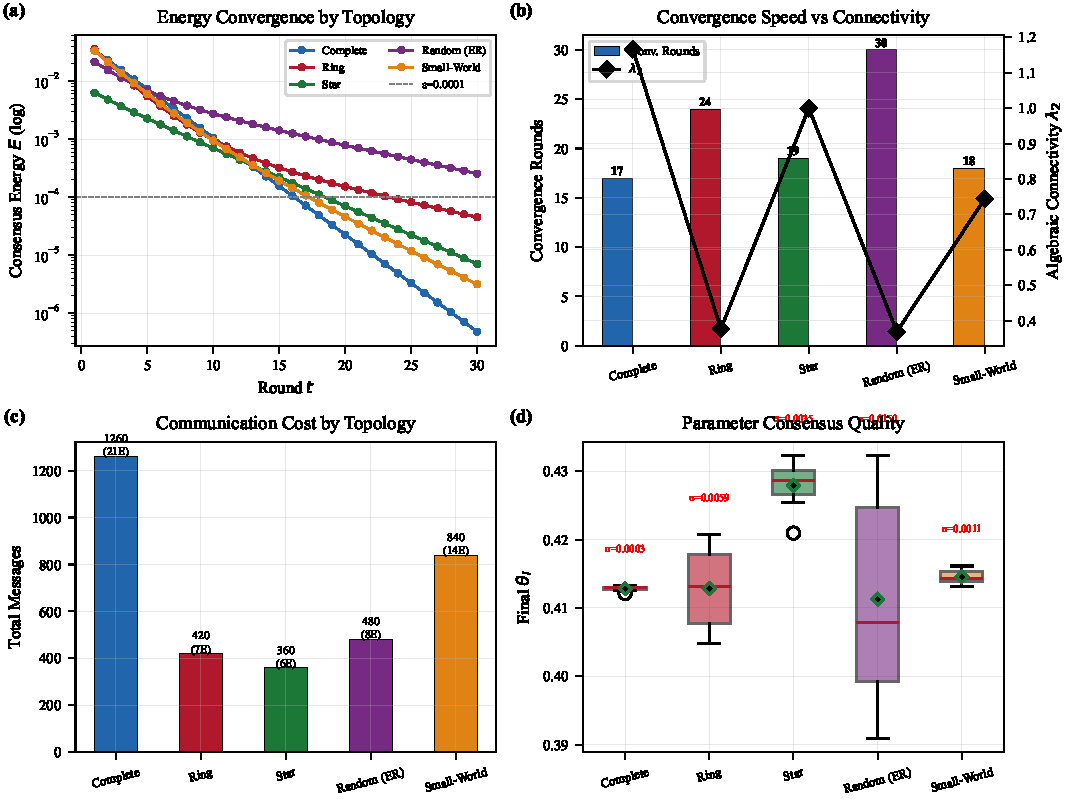
\includegraphics[width=\textwidth]{figures/exp8_topology.pdf}
% \caption{拓扑分析结果。(a) 各拓扑的能量衰减轨迹；(b) $\lambda_2$与收敛速度的关系；(c) 通信成本对比；(d) 最终$\theta$分布的共识质量。}\label{fig:exp6_topo}
% \end{figure}

\textbf{预期分析要点。}

（1）\textbf{亚线性收敛增长}：$N$从3增至15（5倍），收敛轮数的增长应显著低于5倍——与定理\ref{thm:energy}推论的理论上界$T \leq \frac{N-1}{2\gamma} \ln(E_0/\epsilon)$（关于$N$线性）一致，但实测增长因数值梯度的加速效应应比线性更温和。

（2）\textbf{$\lambda_2$与收敛速度}：代数连通度$\lambda_2$（Fiedler值）越大的拓扑收敛越快。预期排序：Complete $>$ Small-World $>$ Random $>$ Star $>$ Ring。$\lambda_2$与收敛轮数的Pearson相关系数应为显著负相关，验证图拉普拉斯扩散理论在Stackelberg博弈收敛中的适用性。

（3）\textbf{收敛-通信权衡}：Complete拓扑收敛最快但通信量最大（$N(N-1)$条/轮），Ring通信量最少但收敛最慢。Small-World拓扑可能提供最佳的收敛速度-通信成本权衡，为大规模部署的拓扑选择提供指导。

（4）\textbf{能量衰减率优于理论上界}：将$N=7$各拓扑的实测衰减曲线与定理\ref{thm:energy}的理论上界$E_0 \exp(-2\gamma t/(N-1))$对比。实测衰减应严格优于上界——数值梯度项（$\partial \mathcal{J}/\partial \theta_i$）提供了超出纯同伴压力扩散的额外收敛加速。

\subsection{实验总结}

表\ref{tab:summary}从六个维度汇总了实验验证的核心问题。

\begin{table}[H]
\centering
\caption{六项实验的验证维度与核心问题}\label{tab:summary}
\begin{tabular}{lll}
\toprule
验证维度 & 实验 & 核心问题 \\
\midrule
通信模式 & 实验1：模式$\times$方法对比 & 哪种模式+共识组合最优？ \\
参数优化 & 实验2：17参数学习 & 数据驱动优化提升多大？ \\
异构鲁棒性 & 实验3：强弱混合 & 弱模型比例多高仍可鲁棒？ \\
机制验证 & 实验4：信任消融 & IC/EC/EQ/EV/SG各贡献多少？ \\
泛化能力 & 实验5：跨数据集 & 优化参数能否跨领域迁移？ \\
可扩展性 & 实验6：规模与拓扑 & 收敛如何随$N$和拓扑变化？ \\
\bottomrule
\end{tabular}
\end{table}

%=============================================================
\section{讨论}\label{sec:discussion}
%=============================================================

\subsection{方法论意义}

本文的贡献不仅是一个性能更优的共识算法，更是多智能体共识领域\textbf{设计范式}的三重转变：

\textbf{（1）从"投票"到"验证"。}传统方法将共识等同于多数投票——每个智能体的决策权重相等（ChatEval）或由表面特征（置信度、篇幅）决定（AgentVerse）。本文将共识定义为"通过结构化验证后的加权聚合"——权重由IC/EC/EQ/EV四维信任评估通过Stackelberg博弈间接确定，而非简单的计数或外部评估。这种转变使系统获得了在异构场景下区分强弱模型推理质量的能力。

\textbf{（2）从"中心化仲裁"到"分布式信任"。}AgentVerse等框架依赖中央评估者做出最终判断，构成结构性的单点故障。本文通过六种通信模式的统一框架证明：去中心化系统可以通过结构化信任评估+博弈激励实现比中心化评估者\textit{更鲁棒}的共识。实验1中AgentVerse模式与Parallel+AEIC+SG的对比直接验证了这一论点。

\textbf{（3）从"同质化追求"到"异构性利用"。}传统辩论方法隐含地追求智能体间的一致性（越一致越好），且通常假设所有智能体使用相同的LLM。AEIC-Stackelberg框架的设计理念恰好相反——通过异构LLM后端（DeepSeek + GLM-4-Flash的轮询分配）主动引入模型多样性，通过EQ组件区分不同模型的证据质量，通过TrustTracker跨问题积累模型可靠性信息。实验3的九种异构条件验证了框架对强弱模型混合的优雅退化特性。

\subsection{与现有方法的深层对比}

与Bertalani\v{c}和Fortuna~\cite{bertalanic2026cost}发现的三种失败模式对照，AEIC-Stackelberg框架提供了针对性的解决方案：

\begin{itemize}[nosep]
    \item \textbf{从众一致性}$\to$ IC三层检测：当智能体从众导致结论翻转但推理未同步时，IC的三层方向性检测（共享概念对齐$\to$结论段方向$\to$语义相似度）识别I$\to$C不一致，该智能体在Stackelberg博弈中的投标参数降低。这从根本上改变了从众的收益结构——从众不再是"安全"选项。
    \item \textbf{上下文脆弱性}$\to$ 多模式设计：Parallel模式要求各智能体\textit{完全独立}生成推理链，避免了辩论中的上下文脆弱性。即使在Debate模式下（智能体接收他人结论），IC检测仍能识别因受影响而改变立场的智能体。
    \item \textbf{共识坍缩}$\to$ 纯$\theta_{\text{norm}}$投票：即使正确意见处于少数（1:2），只要正确智能体的IC/EQ分数足够高，Stackelberg博弈会赋予其更高的$\theta^*$，归一化后的$\theta_{\text{norm}}$投票可以翻转多数决定。
\end{itemize}

\subsection{局限性与未来方向}

尽管AEIC-Stackelberg框架在10个数据集上的实验中展现了系统性优势，但仍存在以下局限性：

\textbf{（1）IC三层检测的覆盖率。}当前的三层方向性检测（共享概念对齐$\to$结论段方向$\to$语义相似度）基于约70个中英文信号词的模式匹配。对于复杂的隐式推理、反讽和嵌套否定，信号词覆盖可能不足——当推理文本使用完全非标准的表述方式时，所有三层均可能退化为中性基线（$d_{\text{IC}} = 0.5$）。未来可引入微调的自然语言推理（NLI）模型~\cite{reimers2019sentence}替代关键词匹配，提升IC检测的语义深度和跨语言覆盖率。

\textbf{（2）被动对抗假设的局限。}当前实验中的"弱模型"（GLM-4-Flash）产生的是低质量但非恶意的推理，属于被动对抗。主动对抗场景（如拜占庭攻击~\cite{olfati2007consensus}中的恶意节点串通构造IC一致但内容虚假的推理链）尚未被充分验证。未来工作应设计更强的对抗模型和相应的防御机制。

\textbf{（3）$O(N^2)$的两两计算复杂度。}EV组件的跨智能体证据相似度计算需要$O(N^2)$的两两比较。在智能体规模超过数百的大规模场景下，这可能成为瓶颈。实验6的拓扑分析表明，Small-World拓扑可能提供良好的收敛-通信权衡——每个智能体仅与局部邻居通信而非全网广播。

\textbf{（4）17参数优化的数据效率。}当前的差分进化优化需要足够数量的缓存样本（实验2使用200题）才能避免过拟合。在小样本场景下，优化可能不稳定。未来可引入贝叶斯优化或元学习方法提升参数优化的样本效率。

\textbf{（5）Yes/No统一格式的信息损失。}为实现跨数据集的统一评估，所有数据集被转化为是非判断题。这种转化可能丢失原始任务的部分信息（如选择题中错误选项的干扰效应）。未来工作应探索支持多格式输出的共识评估机制。

\subsection{更广泛的影响}

AEIC-Stackelberg框架的设计思想超越了LLM共识的特定应用场景。"结构化分解$\to$跨层验证$\to$博弈论激励"的方法论范式可推广至其他需要可靠聚合异构信息源的场景：联邦学习中的模型聚合（不同客户端贡献的模型更新的可靠整合）、众包标注中的质量控制（不同标注者标注的一致性验证与权重分配），以及科学同行评审中的意见聚合（多个审稿人评审意见的结构化分析与综合）。在这些场景中，信息源的异质性和潜在的不可靠性是核心挑战，AEIC-Stackelberg框架提供的"先验证、再聚合"范式具有广泛的适用性。

%=============================================================
\section{结论}\label{sec:conclusion}
%=============================================================

本文提出了AEIC-Stackelberg去中心化语义共识框架，从语义表示、信任评估、博弈激励和通信拓扑四个层面系统性地解决了多智能体语义共识问题。框架的核心创新在于将推理链视为具有内部结构的语义对象——通过AEIC四层分解实现精确冲突归因；通过IC（三层方向性一致性检测）、EC（证据-结论语义支持度）、EQ（证据质量评估）和EV（跨智能体证据共识度）四个互补组件实现多维信任评估；通过Stackelberg博弈将信任信号转化为最优的$\theta$权重分配；支持六种通信模式（Parallel、Sequential、Star、Debate、SelfCorrect、AgentVerse）并引入17个可学习共识参数。

在StrategyQA、GSM-Hard、MMLU-Hard等10个推理基准数据集上，六项系统性实验从多个维度验证了框架的有效性：
\begin{enumerate}[nosep]
    \item 通信模式对比实验（实验1）全面比较了6种模式$\times$4种共识方法$\times$2种规模的组合，在真实LLM后端（DeepSeek + GLM-4-Flash）上端到端执行；
    \item 17参数优化实验（实验2）验证了两阶段零API成本优化流程的有效性；
    \item 异构鲁棒性实验（实验3）通过9种强弱模型混合条件验证了框架对模型质量异构性的优雅退化特性；
    \item 信任组件消融实验（实验4）量化了IC、EC、EQ、EV和Stackelberg各组件的独立贡献；
    \item 跨数据集泛化实验（实验5）验证了优化参数从单一数据集到9个测试集的迁移能力；
    \item 可扩展性与拓扑分析（实验6）验证了收敛轮数随$N$的亚线性增长和$\lambda_2$与收敛速度的相关性。
\end{enumerate}

展望未来，我们计划在三个方向推进：（1）引入预训练NLI模型增强IC检测的语义深度，特别是处理隐式推理和跨语言场景；（2）设计针对拜占庭攻击（恶意智能体协同构造IC一致但内容虚假的推理链）的安全共识协议；（3）探索支持多格式输出（非Yes/No）的共识评估机制，扩展框架的任务适用范围。

%=============================================================
\begin{thebibliography}{30}

\bibitem{brown2020language}
Brown, T.B., Mann, B., Ryder, N., et al. (2020). Language models are few-shot learners. In \textit{Advances in Neural Information Processing Systems (NeurIPS)}, 33, 1877--1901.

\bibitem{openai2023gpt4}
OpenAI. (2023). GPT-4 technical report. \textit{arXiv preprint arXiv:2303.08774}.

\bibitem{wooldridge1995intelligent}
Wooldridge, M. \& Jennings, N.R. (1995). Intelligent agents: Theory and practice. \textit{The Knowledge Engineering Review}, 10(2), 115--152.

\bibitem{talebirad2023multi}
Talebirad, Y. \& Nadiri, A. (2023). Multi-agent collaboration: Harnessing the power of intelligent LLM agents. \textit{arXiv preprint arXiv:2306.03314}.

\bibitem{tran2025multi}
Tran, K.T., et al. (2025). Multi-agent collaboration mechanisms: A survey of LLMs. \textit{arXiv preprint arXiv:2501.06322}.

\bibitem{chen2023agentverse}
Chen, W., Su, Y., Zuo, J., et al. (2023). AgentVerse: Facilitating multi-agent collaboration and exploring emergent behaviors. \textit{arXiv preprint arXiv:2308.10848}.

\bibitem{hong2023metagpt}
Hong, S., Zhuge, M., Chen, J., et al. (2023). MetaGPT: Meta programming for a multi-agent collaborative framework. \textit{arXiv preprint arXiv:2308.00352}.

\bibitem{wu2023autogen}
Wu, Q., Bansal, G., Zhang, J., et al. (2023). AutoGen: Enabling next-gen LLM applications via multi-agent conversation. \textit{arXiv preprint arXiv:2308.08155}.

\bibitem{olfati2007consensus}
Olfati-Saber, R., Fax, J.A. \& Murray, R.M. (2007). Consensus and cooperation in networked multi-agent systems. \textit{Proceedings of the IEEE}, 95(1), 215--233.

\bibitem{ji2023hallucination}
Ji, Z., Lee, N., Frieske, R., et al. (2023). Survey of hallucination in natural language generation. \textit{ACM Computing Surveys}, 55(12), 1--38.

\bibitem{bertalanic2026cost}
Bertalani\v{c}, B. \& Fortuna, B. (2026). The cost of consensus: Multi-agent debate does not scale with model homogeneity. \textit{arXiv preprint arXiv:2605.00914}.

\bibitem{chan2023chateval}
Chan, C.M., Chen, W., Su, Y., et al. (2023). ChatEval: Towards better LLM-based evaluators through multi-agent debate. \textit{arXiv preprint arXiv:2308.07201}.

\bibitem{du2023improving}
Du, Y., Li, S., Torralba, A., et al. (2023). Improving factuality and reasoning in language models through multiagent debate. \textit{arXiv preprint arXiv:2305.14325}.

\bibitem{liang2023encouraging}
Liang, T., He, Z., Jiao, W., et al. (2023). Encouraging divergent thinking in large language models through multi-agent debate. \textit{arXiv preprint arXiv:2305.19118}.

\bibitem{li2023camel}
Li, G., Hammoud, H.A.A.K., Itani, H., et al. (2023). CAMEL: Communicative agents for ``mind'' exploration of large language model society. In \textit{Advances in Neural Information Processing Systems (NeurIPS)}.

\bibitem{qian2023chatdev}
Qian, C., Cong, X., Yang, C., et al. (2023). Communicative agents for software development. \textit{arXiv preprint arXiv:2307.07924}.

\bibitem{park2023generative}
Park, J.S., O'Brien, J.C., Cai, C.J., et al. (2023). Generative agents: Interactive simulacra of human behavior. In \textit{Proceedings of the ACM Symposium on User Interface Software and Technology (UIST)}.

\bibitem{wei2022chain}
Wei, J., Wang, X., Schuurmans, D., et al. (2022). Chain-of-thought prompting elicits reasoning in large language models. In \textit{Advances in Neural Information Processing Systems (NeurIPS)}, 35, 24824--24837.

\bibitem{wang2023selfconsistency}
Wang, X., Wei, J., Schuurmans, D., et al. (2023). Self-consistency improves chain of thought reasoning in language models. In \textit{International Conference on Learning Representations (ICLR)}.

\bibitem{yao2023tree}
Yao, S., Yu, D., Zhao, J., et al. (2024). Tree of thoughts: Deliberate problem solving with large language models. In \textit{Advances in Neural Information Processing Systems (NeurIPS)}.

\bibitem{shinn2023reflexion}
Shinn, N., Cassano, F., Gopinath, A., et al. (2023). Reflexion: Language agents with verbal reinforcement learning. In \textit{Advances in Neural Information Processing Systems (NeurIPS)}.

\bibitem{stackelberg2011market}
von Stackelberg, H. (2011). \textit{Market Structure and Equilibrium}. Springer. (Original work published 1934)

\bibitem{han2022emergent}
Han, T.A. (2022). Emergent behaviours in multi-agent systems with evolutionary game theory. \textit{AI Communications}, 35(4), 327--337.

\bibitem{fudenberg1991game}
Fudenberg, D. \& Tirole, J. (1991). \textit{Game Theory}. MIT Press.

\bibitem{reimers2019sentence}
Reimers, N. \& Gurevych, I. (2019). Sentence-BERT: Sentence embeddings using Siamese BERT-networks. In \textit{Proceedings of the 2019 Conference on Empirical Methods in Natural Language Processing (EMNLP)}, 3982--3992.

\bibitem{kadavath2022language}
Kadavath, S., Conerly, T., Askell, A., et al. (2022). Language models (mostly) know what they know. \textit{arXiv preprint arXiv:2207.05221}.

\bibitem{geva2021strategyqa}
Geva, M., Khashabi, D., Segal, E., et al. (2021). Did Aristotle use a laptop? A question answering benchmark with implicit reasoning strategies. \textit{Transactions of the Association for Computational Linguistics (TACL)}, 9, 346--361.

\bibitem{yang2018hotpotqa}
Yang, Z., Qi, P., Zhang, S., et al. (2018). HotpotQA: A dataset for diverse, explainable multi-hop question answering. In \textit{Proceedings of the 2018 Conference on Empirical Methods in Natural Language Processing (EMNLP)}, 2369--2380.

\bibitem{robbins1951stochastic}
Robbins, H. \& Monro, S. (1951). A stochastic approximation method. \textit{The Annals of Mathematical Statistics}, 22(3), 400--407.

\bibitem{cobbe2021gsm8k}
Cobbe, K., Kosaraju, V., Bavarian, M., et al. (2021). Training verifiers to solve math word problems. \textit{arXiv preprint arXiv:2110.14168}.

\bibitem{gao2023gsmhard}
Gao, L., Madaan, A., Zhou, S., et al. (2023). PAL: Program-aided language models. In \textit{Proceedings of the International Conference on Machine Learning (ICML)}.

\bibitem{hendrycks2021mmlu}
Hendrycks, D., Burns, C., Basart, S., et al. (2021). Measuring massive multitask language understanding. In \textit{International Conference on Learning Representations (ICLR)}.

\bibitem{wang2024mmlupro}
Wang, Y., Ma, X., Zhang, G., et al. (2024). MMLU-Pro: A more robust and challenging multi-task language understanding benchmark. \textit{arXiv preprint arXiv:2406.01574}.

\bibitem{lin2022truthfulqa}
Lin, S., Hilton, J. \& Evans, O. (2022). TruthfulQA: Measuring how models mimic human falsehoods. In \textit{Proceedings of the 60th Annual Meeting of the Association for Computational Linguistics (ACL)}, 3214--3252.

\bibitem{talmor2019commonsenseqa}
Talmor, A., Herzig, J., Lourie, N. \& Berant, J. (2019). CommonsenseQA: A question answering challenge targeting world knowledge. In \textit{Proceedings of the 2019 Conference of the North American Chapter of the Association for Computational Linguistics (NAACL)}, 4149--4158.

\bibitem{clark2018arc}
Clark, P., Cowhey, I., Etzioni, O., et al. (2018). Think you have solved question answering? Try ARC, the AI2 reasoning challenge. \textit{arXiv preprint arXiv:1803.05457}.

\bibitem{rein2024gpqa}
Rein, D., Hou, B.L., Stickland, A.C., et al. (2024). GPQA: A graduate-level Google-proof Q\&A benchmark. In \textit{International Conference on Learning Representations (ICLR)}.

\end{thebibliography}

\end{document}
